\chapter{力}
\section{教学要求}
这一章讲述力的初步知识,为了减少学生开始学习高中
物理时遇到的困难,降低与初中物理的台阶,本章不讲静力学
的知识,只讲学习动力学所必需的预备知识。


这一章的教学要求是:

\begin{enumerate}
\item 正确理解力的概念,认识力是物体对物体的作用;知
道重力、弹力、摩擦力的产生条件以及它们的大小和方向;
掌握倔强系数,会计算弹簧的弹力;掌握滑动摩擦系数,会计
滑动摩擦力。
\item 进一步认识力是物体间的相互作用,掌提牛顿第三
定律。
\item 
初步学会分析物体的受力情况,会画物体受力图。
\item 理解合力和分力的概念,掌握平行四边形法则,知道
三角形法,会用作图法和公式法求合力和分力。
\end{enumerate}

在重力的教学中讲到了物体静止时拉紧悬绳的力或压在
水平支持物上的力,其大小等于物体所受的重力。在这节很
难从道理上把这一点讲清楚,先要求学生作为事实接受下来,
讲过牛顿第三定律后再来解决,这里所以要提到这一点,是
使学生对重力的大小有个具体认识,但主要还是因为在讲牛
顿第三定律之前就要用到它,如在计算摩擦力的习题中,在
测定滑动摩擦系数的学生实验中,都要用到.

弹力的方向问题比较复杂,在中学阶段经常遇到的弹力
大都是支持力和拉力,因此,弹力的方向是就支持力和拉力这
两种情形来讲解的,并要求学生掌握,以便以后进行力的分析。

在讲述胡克定律之前,为了扩展学生的眼界,先就几种基
本的形变定性说明:形变越大,弹力也越大,对金属丝的扭转
形变,说明扭转角度越大,弹力也越大,是考虑到以后讲卡文
迪许扭秤和库仑扭秤时要用到,这里并不要求详细地讨论。胡
克定律是就弹簧的弹力来讲的,给出了倔强系数的概念,但不
要求全面分析它跟弹簧的哪些因素有关,胡克定律的公式写
成$f=kx$, 没有写成$f=-kx$, 是考虑到这里还没有讲一维矢
量的运算,写成前者初学者容易接受;讲到简谐振动时再考虑
弹力的方向,写成后者。

摩擦力的教学,重点是讲述滑动摩擦力,静摩擦的教学,
只要求学生了解静摩擦和最大静擦力的概念,不讲静摩擦系
数。在讲解滑动摩擦时提到相对滑动,在讲解静摩擦时提到
相对运动趋势,只是为了讲解得确切一些,不要求涉及较为复
杂的情形(例如一个物体在传送带上相对滑动或相对静止)来
展开讲解。

讲述物体受力分析,既是教给学生一种分析方法,也是前
面学过的知识的综合运用。考虑到学会物体受力分析要贯穿
在整个力学教学中,本章只限于分析最基本的事例。讲述分
析方法,要强调明确研究的对象,分析时应强调力是物体对物
体的作用。至于按照什么顺序(如按重力、弹力、摩擦力的顺
序)来分析力,不宜过分强调,强调得过分,甚至要求学生死
记住一个分析的顺序,对于学生灵活运用知识,学会分析方
法,都是没有好处的。物体的受力情况实际上往往是很复杂
的,根据具体的问题,可以略去某些次要因素。这种研究问题
的方法,应该作为一项要求向学生提出,在以后作力的分析时
也要注意这一点。

力的合成和分解的教学,主要是使学生掌握力的平行四
边形法则。三角形法在实际中常常用到,学生应当知道。但
应该使学生明确,三角形法并不是另外一种新方法,只是平行
四边形法的简化。


\section{教学建议}
这一章内容,建议在教学中分为三个单元:

第一单元(第1节——第7节)讲述力的概念和力学中常见
的三种力,并在此基础上讲述牛顿第三定律和物体受力情况
分析。

第二单元(第8节——第10节)讲述力的合成和分解.

第三单元(第11节——第12节)在前面讲过的力的矢量性
的基础上,讲述矢量的初步知识。

\subsection{第一单元}
这一单元,首先通过重力、弹力、摩擦力这三种常见的力
和牛顿第三定律的教学,使学生比较具体地认识力的概念和
性质,包括力是物体之间的相互作用,力有大小、方向和作用
点等,然后引导学生初步掌握物体受力情况分析的方法,为进
一步学习力学知识打下基础。

\subsubsection{力的概念和图示}

这部分内容大部分在初中已经学
过,是复习性的。但是有一些学生,虽然能记住学过的知识,
并不真正理解、会用,所以对这部分内容的教学仍然要给予
足够的重视。

力的概念的教学,最主要的是通过演示和说明使学生真
正理解力是物体对物体的作用,只要有力就一定有施力物体
和受力物体,力不能离开物体而存在。这是力学中最基本的
事实。可以通过一些实际的例子让学生指出施力物体和受力
物体,学生牢牢地掌握这一点,就不会离开物体的作用凭空设
想出多余的力来,有助于学好后面的物体受力分析。

关于力的图示,要强调表示力的每条有向线段,都要根据
选择好的标度,按照一定的比例来画。有的同学,往往用不同
的标度来画同一物体所受的不同的力,这种错误应该及时给
予纠正,一般情况下,力的作用点都可画在物体的质心上。由
于教材没有介绍质心这个概念,在实际作图时,只要在表示物
体的图形中间选择一个适当的点来表示力的作用点就可以
了,但是也有个别情况,例如第一次介绍摩擦力的方向时(课
本图1.12),为了清楚起见,把摩擦力$f$画在接触面上,而且
还把相互接触的两个物体画得离开一些。以后还应逐步使学
生知道,在分析力学问题时,有时只须画出力的示意图。力的
示意图常常是为了使物体的受力分析更清楚而作的,它在力
的大小、标度上的要求,不象力的图示中要求的那么严格,但
是对力的方向、力的相对大小也不能画错。在另一些情况下,
例如,在物体的受力分析之后,需作它的受力图并用图示法来
解题,这时的受力图又必须按力的图示的要求来作图了。但
是在本节的教学中,只须按课本上的要求进行就可以了。

\subsubsection{重力} 关于重力的概念,按教材上所讲的“由于地球
的吸引而使物体受到的力叫做重力”来进行教学是适宜的,它
既浅显易懂,也没有把引力与重力等同起来。这里也不宜过
早的把地球对物体的引力与重力相区别,以后在教学中会逐
步讲清楚的。

应该注意的是,教材上把重量定义为物体所受的重力,按
照国务院颁布的法定计量单位,重量是质量的同义词。这种
差别的产生是因为教材是在法定计量单位颁布前编写的。这
一点,在教学中应该向同学们讲清楚。

物体所受重力的大小,可以用静力学的方法来确定,这就
是教材上讲的物体静止时拉紧悬绳的力或压在水平支持物上
的力,它们的大小都跟物体所受的重力相等。应该让学生注
意的是,重力是地球作用在物体上的力,受力者是物体,而物
体对悬绳的拉力或对支持物的压力,受力者是悬绳或支持物,
它们跟重力是作用在不同物体上的力,不能把它们跟重力相
混淆。

重力这一节的教学,也是具体地通过这种常见的力来表
明:力是物体对物体的作用,力有大小、方向和作用点,从而使
学生逐步加深对力这个抽象概念的理解。重心的概念,也是
从重力的概念引伸出来的,因为课本不讲同向平行力的合成,
不要追求概念的严谨,补充重心的定义,通过课本中图1.2
的演示,很容易说明“一个物体的各部分都要受到地球对它的
作用力,我们可以认为重力的作用集中于一点,这一点叫做物
体的重心。”

\subsubsection{形变与弹力}
这一内容的教学,应着重于有关形变与
弹力的实验演示(包括显示微小形变的实验演示),使学生从
直观上来理解和接受,而不宜增加关于形变产生弹力的微观
解释。课本中说明弹力与重力不同,弹力只有在物体直接接
触并产生形变时才能产生。而实际上,有时微小形变又不易
察觉,这样从表观上就不易直接判别出相互接触的物体之间
究竞是否有形变与弹力产生。原则上这里只须提醒同学注意
这个问题,至于进一步具体判断的方法,应在以后学习物体的
平衡等节内容时再作讨论。有关弹力方向的问题,宜按课本
中的提法,即第13页和第14页两段有波纹线的文字,说明支
持力和拉力的方向,由于还存在扭转、切变等种种形变,教学
中不宜笼统地表述为“弹力的方向总是指向……”的形式。

\subsubsection{摩擦力} 摩擦力一节的教学重点是滑动摩擦力,教学
时可在初中学过的知识基础上,通过演示得出关系式$f=\mu N$,
引出滑动摩擦系数的概念,对于这个公式,有的同学往往误
认为压力$N$的大小总是跟滑动物体所受的重力相等,教师
应该让他们知道,压力$N$是跟两个物体的接触面垂直的。只
有物体在水平拉力作用下沿水平面滑动时,压力$N$的大小才
跟物体所受的重力相等,在其他情况下,例如物体沿斜面下滑
时,压力$N$并不等于物体所受的重力。

摩擦力不是教学的重点,在判断静摩擦力的方向时,
同学们对相对运动趋势常常感到比较抽象。在不讨论静摩擦
力作为动力的情况下(如传送带上的物体等),可引导同学这样
来认识:按照已经给定的力来看,物体本是要运动的,但实际
上物体却处于静止状态,那阻碍物体运动的力便是静摩擦力。
这样静摩擦力的方向也就随之而明确了。

\subsubsection{作用力和反作用力}
牛顿第三定律是一个基本定律,
是本章的重点,讲好重点知识,应该引导学生抓住定律的主
要之点。对初学者来说,牛顿第三定律的主要之点就是作用
力和反作用力分别作用在相互作用的两个物体上,教材正是
抓住了这一点,通过实例和演示,反复加以说明,而没有侧重
于作用力和反作用力是同种性质的力,它们同时产生、同时消
失。在教学中应该注意这个问题,不能把主要之点当作自明
之理一带而过,把力量耗费在讲述一些次要问题上。讲解牛
顿第三定律,也是在进一步扩展学生对力的概念的认识,明确
力是物体对物体的相互作用。关于作用力和反作用力跟平衡
力之间的区别,学生常常理论上知道,实际上还会混淆。教学
中要通过一些实例,引导学生搞清两者的区别。例如,可以分
析放在桌面上的静止物体,找出它所受的一对平衡力,以及物
体所受的重力和它对桌面的压力的反作用力,还可以分析用
悬绳挂在天花板下的物体,找出作用在物体和悬线上的平衡
力,以及地球和物体,物体和悬绳、悬绳和天花板间的作用力
和反作用力。当然这个问题也不是一堂课所能解决的,下一
节物体受力分析,还要讨论这类问题。

\subsubsection{物体受力情况分析}  这一节内容,是在以前各节预备
知识的基础上提出的,是前面各节有关知识的应用,这一节内
容的安排也是循序渐近的:从静止物体到运动物体,从平面上
的物体到斜面上的物体,从具体实例上升到分析物体受力情
况的一般方法——隔离法。

在教学上要注意:
\begin{enumerate}
    \item 引导学生正确地搞清楚研究对象,
施力物体与受力物体;
\item 要找到分析对象受到的所有的力,
不能遗漏,但也不能“无中生有”,不能“张冠李戴”;
\item 不能只
讲一般原则和注意事项,不能仅靠课堂上受力分析的示范,还
要行适量的实例练习,画出受力图,及时发现问题,及时引
导同学自觉纠正错误,逐步掌握正确的受力分析方法。
\end{enumerate}

物体受力情况是各种各样的,因此不可能在这一节教学
中要求学生完全掌握,要有一个过程。循序渐进在这里特别
重要,切不可一次就补充很多复杂的题目让同学分析。这样
反而会使同学无所适从,甚至产生畏难情绪。对隔离法的教
学要求尤宜如此,所以课本中没有提出连接体之类的繁难问
题,而把重点放在引导学生理解和掌握受力分析的方法和思
路上。如果学生能掌握正确的方法和思路,则他们自己也会
逐渐独立地解析各种力学题目。

在受力分析时,常常忽略某些次要因素,这也是使所研究
的问题理想化,应该在教学中引导同学重视并逐渐熟悉这种
方法。例如物体下落时,相对于重力来说,可以忽略空气阻力
这一次要因素,通过理想化才构成了自由落体运动这一模型。
以后的教学中还要不止一次地运用这种方法,使本来很复杂
的问题,能够较容易地入手研究。当然这些话并不是都要在
这节课中向学生一一说明的。

\subsection{第二单元}
这一单元讲力的合成和分解,主要使学生掌握力的平行
四边形法则。这个法则是进行力学计算的基本规律,是本章
的叉一重点,由于学生初次接触这种运算,很不习惯,因此也
是难点。教学中应该通过演示,实验和力的图示,使学生理解
和掌握这一规律。

\subsubsection{力的合成}
在讲合力和力的合成的概念时,首先要从
生活中的事例出发,让学生理解儿个力共同作用的效果可以
跟另外一个力单独作用的效果相同,例如,一件行李,可以由
两个人共同提,也可以由一个人提;吊起一个重物,可以用两
根悬绳,也可以只用一根悬绳;一辆车子,可以由几个人推着
它匀速前进,也可以由一个人推着它匀速前进,等等,然后再
引入合力和力的合成的概念,这可以使抽象的概念具体化,便
于学生理解.力的平行四边形法则的教学,做好课本中图1.
22的演示实验是个关键。可以把实验装置装在竖立的小黑
板上,边讲边画出力的图示,还要事先设计好几组不同的数
据,不要只由一次实验的结果就总结出规律来。在处理力的
三角形法时,可以只把它当作代替力的平行四边形法则的简
单的作图法,介绍三角形法时,要学生搞清楚“首尾相接”的
意思,以免把合力的方向搞错,有的同学对于合力跟分力之
间的关系认识不清,学了力的合成以后,往往认为物体在受
到几个力作用的同时,还要受到它们的合力的作用。这种错
误认识应该纠正,要使学生认识,合力与分力之间是等效“代
替”的关系,而不是合力跟分力同时作用在物体上。

\subsubsection{力的分解}   在讲力的分解时,也要通过实例和演示,
使学生体会:一个力往往可以产生几个效果。例如,在同一悬
点上,用两根悬绳吊起一个物体,物体对悬点的竖直向下的
拉力,产生了同时拉紧两根悬绳的效果,由此可以引出分力
和力的分解的概念。

在讲述怎样分解一个力时,教材是通过两个实际的例子,
得出一个力可以根据它产生的效果进行分解的结论,在这里,
教材上的提法是谨慎的、留有余地的。因为在许多情况下,力
的分解不是根据它产生的实际效果,而是要按照研究问题的
方便来进行的,大家熟知的力的正交分解法就是一个很好的
例子。

\subsection{第三单元}
这个单元是在前两个单元的知识基础上,提出矢量的概
念,并学习同一直线上的矢量的运算方法,为以后直线运动中
位移和速度的合成提供了依据。

\subsubsection{矢量与标量} 
这节教材的教学,主要在于讲清楚矢量
与标量的不同含义和不同运算法则。这里从力的合成要按照
平行四边形法则来进行,外推到平行四边形法则也是矢量合
成(矢量加法运算)的普遍法则就够了,无须再举例展开,矢
量与标量在运算规则上的不同,教学中也只举加法运算为例,
至于矢量的减法和乘、除运算就更不须提出来进行比较了。

\subsubsection{一维矢量运算}  在同一直线上的矢量的运算,是矢量
运算中最简单的情况,在讲过一般的矢量加法运算之后,在这
里作较为详细讲述,是因为以后讲直线运动时要用到这一知
识,要着重讲清:先要沿着矢量所在的直线选定一个正方向,
规定凡是方向跟正方向相同的矢量都取正值,凡是方向跟正
方向相反的矢量都取负值。这样,就可以用一个带有正负号的
数值把矢量的大小和方向都表示出来,从而把同一直线上的
矢量运算简化为代数运算,为下一章直线运动中位移和速度
的运算提供了很大的方便。教学中应该引导学生重视这一节
内容并仔细阅读认真领会课文,要弄清楚课本上说的“可以用
一个带有正负号的数值把矢量的大小和方向都表示出来”的
含义,是把矢量的大小和方向分开来表示的.例如$F=-6$牛,
力的大小用数值和单位(6牛)表示,而力的方向则按跟预先
规定的正方向相同或相反(取正号或负号)来表示,掌提了
这个基本点,一维矢量的运算就容易弄清楚了。

\section{实验指导}
\subsection{演示实验}
\subsubsection{重心的实验测定方法}
在演示课本图1.4所介绍的用悬挂法测物体的重心位置
时,应使学生明确:
\begin{enumerate}
\item 利用这种方法测重心只能用于薄板状(即厚度极小
可以忽略)的物体,任何有厚度的物体的重心不会在物体的某
一个表面上。
\item 重心可以不在物体上,如用悬挂法可以测出一个薄
板状的塑料衣架的重心$C$并不在衣架上(图1.1)。一个薄板
状的圆环的重心一定在环心上。
\end{enumerate}

\begin{figure}[htp]
    \centering
\includegraphics[scale=.8]{fig/1-1.png}
    \caption{}
\end{figure}


\subsubsection{物体形变时产生的弹力}
在做课本图1.5的实验时,为了突出所观察的是一端固
定的弹簧被拉长和被压缩时所产生的弹力对小车的作用,小
车上不必加放砝码,以免分散学生的注意力。如果为了使效
果明显可用倔强系数较小的弹簧。

课本图1.6所示的现象,要用较大的、一侧透明的水槽,
圆木的质量又必须足够大,一般不容易演示,如果用投影仪,
则不易看清细木棍的弯曲形变的恢复过程,因此建议改用细
木条(用制作模型飞机的木条$1\x2\x300 {\rm mm}^3$)把一辆原来静
止的小车推开的现象来演示。

演示课本图1.7的现象时,可用洗澡用的或做沙发床垫
用的塑料,观察发生形变和形变的恢复,效果较好。

\subsubsection{显示微小形变的实验装置}
可按课本图1.10的装置进行演示,为了使效果明显,应
使两块平面镜$M$和$N$间的距离相隔得尽可能远些,屏幕可
利用教室的墙壁,以便离开平面镜$N$的距离更大些。如果用
激光作为光源,在教室内就可演示。如果用白炽灯制成的平
行光源,则需在作为屏幕的墙的一边,用黑窗帘(或黑纸)把窗
户局部遮光。

这一装置是利用光在均匀媒质中的直线传播和平面镜组
对于光线的二次反射原理制成的,在入射光线的方向不改变
的情况下,如果平面镜转过$\theta$角,则反射光线将偏转$2\theta$角(图
1.2),当在桌面上施加一个压力,桌面发生微小的弯曲形变
时,两块原来平行放置的平面镜就不再平行了,$M$将向左侧
偏斜一个微小角度$\theta$, $N$将向右侧偏斜一个微小角度.由
于$M$的偏斜,使得反射角变小了$2\theta$. 对平面镜$N$来说,入射
光线的方向已发生了变化,又由于$N$的偏斜,使得入射角比原
来减小了$2\theta- \theta'$. 于是从$N$反射的光线的偏离程度就更大。
即反射角将变小$2(2\theta+\theta')$. 再加上由于屏幕离$N$的距离$r$
较远,即使$\theta$和$\theta'$都十分微小,光点在屏幕上的移动距离$\Delta s\approx r\x 2(2\theta+\theta')$仍是十分明显的,这种利用光线的二次反射
把微小效应放大的作用,常称为“光杠杆的放大作用”。
\begin{figure}[htp]\centering
    \begin{minipage}[t]{0.48\textwidth}
    \centering
\includegraphics[scale=.7]{fig/1-2.png}
    \caption{}
    \end{minipage}
    \begin{minipage}[t]{0.48\textwidth}
    \centering
    \includegraphics[scale=.7]{fig/1-3.png}
    \caption{}
    \end{minipage}
    \end{figure}

\subsubsection{扭转形变}
课本图1.11所示的扭转形变,可用直径为20—25毫米
的橡皮管进行演示,沿着管轴方向平行地用颜色漆划几条线,
在橡皮管的两端各塞上一小段圆木,把管子的一端用试管夹
固定起来,在另一端用一根粗铁丝沿塞子的直径方向穿过(图
1.3)。这样,当在铁丝上加一力偶使它转过一个角度时,就可
明显地显示出扭转形变。


\subsubsection{静摩擦和滑动摩擦}
如图1.4所示,先用水平仪把长木板调节水平,并调节滑
轮$P$或调节固定在木块$B$上的钩子$C$的位置,使得细绳被拉
直时与长木板表面平行。在砝码盘$A$中加一小砝码,木块$B$
仍能保持静止。通过对木块$B$进行受力情况的分析,说明静
摩擦力的存在,然后在砝码盘$A$中逐渐增加砝码,直到$B$开始
运动。这说明在木块开始运动之前所受到的静摩擦力是随着
细绳拉力的增大而增大的,但静摩擦力的增大有一限度,即存
在一个最大静摩擦力。
\begin{figure}[htp]
    \centering
    \includegraphics[scale=.7]{fig/1-4.png}
    \caption{}
\end{figure}

适当调整盘中砝码的数量,使得木块$B$能沿着长木板做
匀速直线运动(不要求很精确,只要大致是做匀速运动就可以
了),通过对木块$B$进行受力情况的分析,可知木块所受到的
滑动摩擦力的大小等于细绳的拉力。通过对砝码盘$A$(连同
其中的砝码)的受力分析,可知细绳的拉力等于盘和盘中所加
砝码所受重的和,从而可知这时木块所受到的滑动摩擦力
的大小就等于盘$A$和盘中砝码所受重力的和。

在木块$B$上加一大砝码(100克或200克),必须重新调
整盘中砝码的数量,才能使$B$做匀速直线运动,测出增大了
压力后滑动摩擦力的数值,由此可说明滑动摩擦力的大小是
跟接触面间的压力大小有关。

在木块$B$的另一个面上事先贴好一张比较粗糙的纸,再
用这个粗糙面跟木板接触,重做实验,发现必须重新调整盘中
砝码的数量,才能使$B$做匀速直线运动。这说明在压力不变
的情况下,滑动摩擦力的大小还跟接触面的材料性质和粗糙
程度有关。

\subsubsection{作用力和反作用力}
课本图1.13的实验在课堂上不能做,可以要求学生
在划船活动时有意识地进行。在课堂教学中可以用两辆小平
板车,请两位学生蹲在小车上,面对面地用手互相推动,来观
察两辆小车互相被推开,向相反方向运动的情况,演示时可
让甲同学将手掌对着乙同学,由乙同学推甲同学的手;再让乙
同学将手掌伸向甲同学,由甲同学施力于乙同学;最后再由
甲、乙两同学同时通过手掌施力于对方。可以观察到这三种
情况下,小车的运动情况是相同的。

课本图1.14的现象要用投影仪来观察,所用的小磁
铁和铁块的质量要相近,但不要太大,软木塞要用大些的,不
然由于重心较高,在软木塞运动过程中磁铁(或铁块)可能会
翻落下去,也可以将磁铁和铁块分别用细线缚在软木塞上,并
且都把它们翻过来放置,让磁铁和铁块在水中相互吸引,这在
投影时的效果是相同的。

为了便于直接观察,也可以用一块较大的条形磁铁和一
块质量相近的铁块,分别在它们的下面垫放几支粉笔(如果粉
笔是圆台形的,刚应将粉笔粗的一端和细的一端交错放置)以
减少摩擦,直接在讲台上演示,效果很明显。演示时可先将磁
铁用手按住,使铁块接近到某一适当距离,可观察到铁块被吸
引过来;再将铁块按住,使磁铁接近到某一适当距离,可观察
到磁铁被吸引过来;然后再将两手控制住磁铁和铁块,调节它
们之间的距离,同时将手放开,可观察到磁铁和铁块相互吸
引,彼此靠近直到吸在一起,这一演示说明了力是物体与物
体间的相互作用,任何施力物体也必然是受力物体。

课本图1.15的实验定量地说明了作用力和反作用
力的关系,是讲解牛顿第三定律的实验基础。在进行这个实验
之前,事先应做好准备,试一下这两个弹簧秤的钩子勾在一起
沿水平方向拉动时,两个弹簧秤的示数是否总是相等。'为了
增加可见度,可在弹簧秤的指示器上贴两块小纸。

将一玩具汽车(电动的或弹簧发条的)放在一块较大
的泡沫塑料平板上,平板下面垫放若干玻璃试管以减小摩擦。
当汽车开动时,可观察到塑料
平板向相反方向运动(图1.5),
说明物体间的摩擦力也是相互作用的。
\begin{figure}[htp]
    \centering
    \includegraphics[scale=.8]{fig/1-5.png}
    \caption{}
\end{figure}

\subsubsection{力的合成的平行四边形法则}
课本图1.22的实验,为了便于计算,可使$F_1$等于三个等
重钩码的重量,使$F_2$等于四个等重钩码的重量,并使当拉绳
的结点到达位置$O$时,两根细绳的夹角恰为$90^{\circ}$, 于是可认为
这两个共点力$F_1$和$F_2$的方向夹角为$90^{\circ}$, 在这两个力的共同
作用下,使橡皮条发生了长度为$EO$的伸长形变。

当演示用一个定滑轮和一组钩码,通过细绳拉橡皮条使
之发生相同的伸长形变时,可以逐次增加钩码,一直加到五个
钩码,可以看到结点恰好到达位置$O$, 加到第六个钩码时结点
已超过位置$O$, 或者可以先加七个钩码,观察结点已远远超过
位置$O$, 然后逐步减少钩码数,直到还剩五个钩码时,观察结
点恰到达位置$O$. 于是这五个钩码所引起的绳子拉力就等于
合力的大小。

\subsubsection{合力的大小跟分力夹角的关系}
课本36页最后有一段文字叙述:“当$F_1$和$F_2$的夹角$\theta$在
$0^{\circ}$到$180^{\circ}$之间时,$\theta$越大,$\cos\theta$的值就越小,合力就越小,而且
合力的方向也随着夹角$\theta$的变化而变化.”关于这一段叙述,
除了从合力的计算式$F=\sqrt{F^2_1+F^2_2+2F_1F_2\cos\theta}$来加以理解
外,还可以用如下的模拟演示来获得感性认识。
\begin{figure}[htp]
    \centering
    \includegraphics{fig/1-6.png}
    \caption{}
\end{figure}


先让学生参阅课本图1.23丙用三角形法来表示共点力
$F_1$和$F_2$的合力$F$, 然后将模拟演示仪介绍给学生,这是用五
合板(或2—2.5毫米厚的有机玻璃)制成的两根长度不等的
箭头,分别用来代表分力$F_1$和$F_2$, 并设$F_1>F_2$. 根据三角形
法,将$F_1$的始端和$F_2$的末端用铆钉铆
合在一起(不要铆死,使它能转动),在$F_1$
的末端和$F_2$的始端间固定一根橡皮条(或宽紧带)用来表示合力(图1.6)。橡皮条的原长应为$F_1-F_2$. 演示时可从$F_1$和$F_2$的夹角$\theta=0^{\circ}$开始,逐渐增大,直到
$\theta=180^{\circ}$. 在这过程中可以看到橡皮条的长度(表示合力$F$的
大小)从$F=F_1+F_2$逐渐减小到$F=F_1-F_2$, 如图1.7所示.
\begin{figure}[htp]
    \centering
    \includegraphics[scale=.8]{fig/1-7.png}
    \caption{}
\end{figure}
因此在两个共点力大小不变的情况下,它们的合力大小是随
着分力夹角的增大而变小的。

\subsubsection{力的分解}
力的分解的演示实际上都是利用二力平衡的原理来显示
的。

(1)课本图1.29,放在斜面上的物体的重力分解。
在一个倾角约为$15^{\circ}$的光滑斜面上,放一辆质量约为200
克的金属小车,小车的一端用细绳跟固定在斜面顶端的弹簧
秤$A$相连(图1.8)。用手托住弹簧秤外壳使它跟斜面平行,观
察这时弹簧秤的示数。将斜面倾角逐渐增大,可以观察到弹簧
秤示数也逐渐增大,当斜面倾角到达$30^{\circ}$时,可读得弹簧秤示
数约为100克力。这说明放在斜面上的物体的重力所产生的一
个效果是使物体沿着斜面下滑,而且斜面倾角越大,使物体沿
斜面下滑的重力分力$F_1$也越大.
\begin{figure}[htp]
    \centering
    \includegraphics[scale=.8]{fig/1-8.png}
    \caption{}
\end{figure}

如图1.9所示,再用一个
铁架台,在复夹上固定另一个
弹簧秤$B$, 通过细绳钩住小车
的中部,在不改变斜面倾角、使
弹簧秤$A$的示数不变的条件
下,调节铁架台的位置和复夹
的高度,使弹簧秤$B$的拉绳方向跟斜面垂直,且使拉绳逐渐绷
紧,直到使小车不对斜面施加压力(即小车刚脱离斜面)。这时
从弹簧秤$B$的示数就可以知道放在斜面上的物体的又一个效
果是使物体紧压在斜面上,可读得斜面倾角为$30^{\circ}$时弹簧秤
$B$的示数约为170克力.
\begin{figure}[htp]
    \centering
    \includegraphics[scale=.8]{fig/1-9.png}
    \caption{}
\end{figure}

如果在这基础上,使斜面倾角继续增大,则可观察到弹簧
秤$A$的示数逐渐增大,弹簧秤$B$的示数逐渐减小。在这过程
中,需要不断调节铁架台的位置和复夹的高度,使得弹簧秤$B$
的拉绳方向始终保持跟斜面垂直。当使斜面的倾角继续增大
到$90^{\circ}$时,可观察到弹簧秤$A$的示数增大到等于小车重量,而
弹簧秤$B$的示数逐渐减小到等于零。当使斜面的倾角逐渐减
小到$0^{\circ}$时,弹簧秤$A$的示数也减小到零,而弹簧秤$B$的示数
将增大到等于小车的重量。

从这个实验可以说明,重力$G$的平行于斜面方向的分力
$F_1=G\sin\theta$, 它的作用效果是使物体沿斜面下滑;重力$G$的
垂直于斜面方向的分力$F_2=G\cos\theta$,它的作用效果是使物体
紧压在斜面上。

(2)课本图1.30, 直角支架的端点所受向下作用力的
分解。

如图1.10所示,直角支架的横梁$OM$是一根装有压缩
弹簧测力计的金属管,$M$端有一套环,可以套在通过复夹安装
在铁架台上的固定转动轴上;斜梁$ON$可用细绳连接弹簧秤
组成,弹簧秤的圆环钩在铁架台上侧的复夹$N$处,细绳的下
端固定在横梁端点$O$处.当在$O$点悬挂重物$G$时,可观察到
细绳被拉紧、横梁被压缩,从弹簧秤和测力计分别可以读出
拉力和压力的数值。这个实验说明了支架$O$点受到一个向下
的作用力$F$时,它对支架的两个梁产生的效果是不同的。
\begin{figure}[htp]
    \centering
    \includegraphics[scale=.8]{fig/1-10.png}
    \caption{}
\end{figure}

演示时,应先调节细绳的长度使得横梁$OM$稍向上倾
斜.这样,当在$O$点挂上重物时,恰好使横梁保持水平,才能
应用直角三角形关系来表示$F$的两个分力$F_1$和$F_2$的大小,
即$F_1=\frac{F}{\cos\theta}$
(它的作用效果使斜梁$ON$受到拉力),$F_2=F\tan\theta$
(它的作用效果使横梁$OM$受到压力)。
\begin{figure}[htp]
    \centering
    \includegraphics[scale=.8]{fig/1-11.png}
    \caption{}
\end{figure}

如果没有压缩弹簧测方计,则可以用另一根细绳在相反
方何通过弹簧秤$C$来拉$O$端,使得$OM$恰巧不变压力,用这
样的方法来进行间接测量(图1.11)。具体做法如下:

用一小方木块$D$, 在它的上部、下部和右侧各装一小钩并
都系上一段细线。上部的细线和弹簧秤$A$相连,下部的细线
悬挂重物,右侧的细线可以系在弹簧秤$C$上。横梁$OM$可用
一根木棒来做,横梁左端装一套环,右端锯成齿状,小木块$D$
的左侧也锯成齿状以增大摩擦,演示时可用手捏住小木块$D$
和横梁的右端不使松动,挂上重物后,由干摩擦,小木块不会
滑动,这时可观察斜梁$ON$受拉力的情况(细线被拉紧),从弹
簧秤$A$可以读出拉力的大小;至于横梁$OM$受压力的情况,
则可间接地用弹簧秤$C$, 通过小木块$D$右侧钩上的细绳,保
持水平地慢慢地拉动,直到横梁不受压力由于自身重力作用,
将会离开小木块$D$而转动,读得这时弹簧秤$C$的示数即为横
梁所受的压力.这个演示同样可以证明当没有用弹簧秤$O$拉
小木块$D$时,横梁$OM$确是受到压力作用的。

\subsection{学生实验}
\subsubsection{测量滑动摩擦系数}

这个实验的目的是定量地测定两种木料之间的滑动
摩擦系数。如何处理实验数据,不宜作过细的规定,可以让学
生复习第一个实验(练习分析处理实验数据),由学生自行设
计表格,进行数据分析和处理。

实验时必须首先利用水平仪把长木板调成水平,而
且要调节滑轮的高度(或调节小木块上钩往细绳的钩子的
位置),使得拉小木块的细绳和长木板保持平行。在这样的情
况下,当小木块沿长木板作匀速运动时,它所受到的滑动摩擦
力$f$的大小,才可以用挂在绳端的砝码盘和盘中砝码受到的
重力之和来量度。

用弹簧秤称出小木块的重量,就求出了压力$N$. 要改变
压力的大小,只要往小木块上加放砝码就可以了。

测得在一系列不同压力时的滑动摩擦力的大小后,
如果利用画图象的方法(不一定用这个方法)来找出它们之间
的定量关系,则可启发学生思考:
\begin{enumerate}
\item 这个实验中的压力和滑动摩擦力这两个物理量,哪
个是自变量,哪一个是因变量?
\item 画图象时平面直角坐标的横坐标应表示哪一个物理
量,纵坐标应表示哪一个物理量?
\item 画出图象后,应怎样得出滑动摩擦系数?
\item 滑动摩擦系数是否有单位?
\end{enumerate}

实验后还可思考以下问题:
\begin{enumerate}
    \item 滑动摩擦力的大小跟压力有怎样的关系?
    \item 滑动摩擦系数的大小是由什么因素决定的?是否可以
    说滑动摩擦系数跟摩擦力成正比,跟压力成反比?压力发生
    了变化,滑动摩擦系数是否会有相应的变化?
    \item 我国东北农村的一些地区,在冬季里人们乘坐的爬
    犁,用几匹狗就可以拉着在雪地里奔驰,如果到了夏季把爬犁
    放在泥地上拉动就很困难,这是为什么?
\end{enumerate}

\subsubsection{互成角度的两个力的合成}

这是一个验证性的实验,在已知两个互成角度的共
点力的情况下,先用力的平行四边形法则求出它们的合力,然
后再用弹簧秤来进行验证。

在实验前可以先把所用的两个弹簧秤的钩子互相钩
住,平放在桌上向相反方向拉动,看看它们的示数在拉力的大
小改变时是否总是相同的。如果是相同的,在实验时就可以
同时使用这两个弹簧秤进行读数。如果不相同,则可以只用
其中一个弹簧秤进行读数(每一个分力或两个分力的合力,都
用这同一个弹簧秤来读数)。

用两个弹簧秤同时拉动一端固定的橡皮条时(要注
意不使伸长量太大,以免用一个弹簧秤测合力时由于超出它
的测量范围而无法读数),要使两个弹簧秤贴着方木板平拉,
弹簧秤互成的角度可以是任意的。但为了便于作图,可以使
两个弹簧秤拉着的细绳沿着一块三角板的任一特殊角(如
$30^{\circ}$、$45^{\circ}$或$60^{\circ}$等)拉动,使橡皮条的另一端伸长到某一位置
$O$. 用细铅笔描下两条细绳的方向,记下两条细绳端点的位
置$O$以及两个弹簧秤的读数$F_1$和$F_2$, 按相同比例(所选定
的标度要在记录纸上明确画出)作出这两个互成角度的共点
力$F_1$和$F_2$的图示,它们的共同作用点也就是绳子的结点位
置$O$.

作平行四边形求出$F_1$和$F_2$的合力$F$时,要求学生
认真地用三角板来作平行线,然后用同一标度量出合力$F$的
大小。

只用一个弹簧秤来拉橡皮条时,可启发学生思考为
什么要使细绳结点拉到同一位置$O$, 这时弹簧秤的读数$F'$和
用两个弹簧秤拉橡皮条时的合力$F$应该有怎样的关系?

用细铅笔描下这时细绳的方向,记下$F'$, 并按相同
的标度在同一力图上画出$F'$的图示。

对有兴趣的学生可以让他们按课本
342页最后一段的叙述进行实验,此外还可
指导他们对刚才实验中的误差进行分析。

比较$F'$和$F$就可以知道误差的大小,如图1.12所示,线段$CC'$就是合力$F'$和$F$之间的误差,线段$CC'$越长,表示误差越大。

\begin{figure}[htp]
    \centering
    \includegraphics[scale=.8]{fig/1-12.png}
    \caption{}
\end{figure}

\subsection{课外实验活动}
\subsubsection{测量尼龙丝的抗断拉力}
这个课外实验是利用最简单的仪器,根据学生所学过的
力的合成和分解的知识,来测量尼龙丝的抗断拉力。

要使学生知道什么是抗断拉力.一段材料发生拉伸
形变对物体产生的弹力是随形变的增大而增大,但是任何材
料对物体产生的弹力都有一个最大值,当材料将被拉断时对
物体产生的最大弹力就是材料的抗断拉力。各种不同材料的
抗断拉力是不同的。

{实验的原理} 

从课本362页图 10.22可知,在尼龙丝的中点悬挂了质
量为1千克的重物,使中点$O$受到向下的力$F=C$, 根据力的
平行四边形法则可知,力$F$跟$F$沿着被拉紧的尼龙丝方向的
分力$F_1$间存在这样的关系:$F=2F_1\cos\frac{\alpha}{2}$(图1.13), 因此将
绳子的另一端沿箭头$\alpha$所示的方向,保持水平地缓慢拉动,随
着。角的逐渐增大,分力$F_1$也逐渐增大,用量角器量出尼龙
丝刚被拉断时的$\alpha$角,就可计算出分力$F$, 而这时的大小
也就等于尼龙丝对$O$点的弹力,于是便可测得尼龙丝的抗断
拉力。

\begin{figure}[htp]
    \centering
    \includegraphics[scale=.8]{fig/1-13.png}
    \caption{}
\end{figure}

实验时的注意事项
\begin{enumerate}
\item 尼龙丝要用很细的一种,不然不易拉断.
\item 将重物悬挂在尼龙丝的中点时,可以通过 一个拉窗
帘用的小环来悬挂,即不要把悬挂重物的细绳在尼龙丝的中
点$O$处打结(打结后就变成两段尼龙丝了)。这样,即使将尼
龙丝的另一端拉动时不在水平方向,由于小环可以滑动,使得
力的合成的平行四边形始终是一个菱形,尼龙丝中的拉力和
向下力的关系仍可满足上述关系式
\item 在拉尼龙丝时可在手指上缠一些布条以免拉紧尼龙丝时会把手指捋破。另一只手可拿着量角器,并使量角器的
圆心始终位于尼龙丝的中点,而且量角器的零刻度始终跟右
侧的尼龙丝重合,如图1.14所示.这样,当尼龙丝被拉断时
就可以方便地读出$\alpha$角的大小。


\begin{figure}[htp]
    \centering
    \includegraphics[scale=.8]{fig/1-14.png}
    \caption{}
\end{figure}


\item 参考数据:如果尼龙丝的直径为0.125毫米,在它的
中点所挂重物的重量为1千克力,当$\alpha=130^{\circ}$时,尼龙丝将被
拉断,则测得抗断拉力
\[F_1=\frac{F}{2\cos\frac{\alpha}{2}}=\frac{1}{2\x \cos65^{\circ}}=1.18\text{千克力}\]

如果找不到尼龙丝,也可以用缝纫机上使用的细线进行
测量。
\end{enumerate}

在实验室中测量尼龙丝的抗断拉力,所用的最方便而
且直接的方法是:把尼龙丝的一端固定,另一端套在一个大量
程的测力计的钩环上,然后将尼龙丝水平地拉紧,并逐渐增大
所施加的拉力,同时观察测力计示数的变化,直到尼龙丝被拉
断,记下这时测力计的读数,就等于尼龙丝的抗断拉力。

也可采用这样的方法:将尼龙丝的上端固定,在其下端悬
挂砝码,并且逐渐增大所加砝码的重量,直到尼龙丝被拉断,
记下这时所加砝码的总重量,就等于尼龙丝的抗断拉力。

\section{习题解答}

\subsection{练习一}
\begin{enumerate}
\item  举出几个实例来说明力是物体对物体的作用.

\begin{solution}
    这样的例子可以举出很多。用铁锤钉钉子,铁锤对
锤子施了力;用手推墙壁,人手对墙壁施了力;跳水运动员用
力蹬跳板,运动员的脚对跳板施了力;汽车停在路面上,车轮
对路面施了力,等等。
\end{solution}
\item 放在水平面上的物体(课本图1.8甲)受到几个力的作用?
  各是什么物体对它的作用,是哪种力?画出物体受力的示意
  图.

  \begin{solution}
    放在水平面上的物体受到两个力的作用,如图1.15
    所示,一个是地球对它作用的重力$G$, 方向竖直向下;一个是
    水平面对它作用的支持力$N$, 方向竖直向上,支持力是弹力。
  \end{solution}
\item 用一根绳子把小球挂在天花板上(课本图1.9甲),小球受
  到几个力的作用?各是什么物体对它的作用,是哪种力?画出
  小球受力的示意图.

  \begin{solution}
    用一根绳子把小球挂在天花板上,小球受到两个力
    的作用,如图1.16所示,一个是地球对它作用的重力$G$, 方
    向竖直向下;一个是绳子对它的拉力$F$, 方向竖直向上,拉力
    是弹力。
  \end{solution}

  \begin{figure}[htp]\centering
    \begin{minipage}[t]{0.32\textwidth}
    \centering
\begin{tikzpicture}[>=latex, scale=1]
\fill [pattern=north east lines] (0,0) rectangle (2,.2);
\draw(0,0.2)--(2,.2);
\draw (.5,.2) rectangle (1.5,.8);
\draw[<->, thick](1,1.5)node[above]{$N$}--(1,.5)--(1,-.5)node[below]{$G$};
\tkzDrawPoint(1,.5)
    \end{tikzpicture}
    \caption{}
    \end{minipage}
        \begin{minipage}[t]{0.32\textwidth}
    \centering
\begin{tikzpicture}[>=latex, scale=1]
    \fill [pattern=north east lines] (0.5,2) rectangle (1.5,2.2);
    \draw(0.5,2)--(1.5,2); 
    \draw(1,2)--(1,.5);\draw[->, thick](1,.5)--(1,1.5)node[right]{$F$};
    \draw[fill=white] (1,.5) circle (.2);
    \tkzDrawPoint(1,.5)
\draw[->,thick](1,.5)--(1,-.5)node[below]{$G$};
    \end{tikzpicture}
    \caption{}
    \end{minipage}
    \begin{minipage}[t]{0.32\textwidth}
    \centering
    \begin{tikzpicture}[>=latex, scale=1]
\fill [pattern=north east lines] (-1,2) rectangle (-1.5,2.2);
    \draw(-1,2)--(-1.5,2); 
\fill [pattern=north east lines] (1,2) rectangle (1.5,2.2);
    \draw(1.5,2)--(1,2); 
\draw(-1.2,2)--(0,.2)--(1.2,2);
\draw(-.3,-.2) rectangle (.3,.2);
\tkzDrawPoint(0,0)
\draw[->,thick](0,0)--(0,-1)node[below]{$G$};
\draw[->,thick](0,.2)--(-.6,1.1)node[left]{$F_1$};
\draw[->,thick](0,.2)--(.6,1.1)node[right]{$F_2$};
    \end{tikzpicture}
    \caption{}
    \end{minipage}
    \end{figure}

\item 用两根绳子把物体挂在天花板上(课本图1.9乙),这个物
  体受到几个力的作用?各是什么物体对它的作用,是哪种力?
  画出物体受力的示意图.

  \begin{solution}
    用两根绳子把物体挂在天花板上,这个物体受到三
    个力的作用,如图1.17所示.
    一个是地球对它作用的重力
    $G$, 方向竖直向下;一个是左边
    绳子对它的拉力$F_1$, 方向沿着
    左边的绳子斜向上;另一个是右边绳子对它的拉力$F_2$, 方向
    沿着右边的绳子斜向上。两根绳子的拉力都是弹力。
  \end{solution}
 \item 找一个薄板状的物体,用书中所讲的悬挂方法求出
  这个物体的重心.

  \begin{solution}
    (略)
    说明:本题是实验题,应该要求学生动手去做。
  \end{solution}
 \item 放在水平桌面上的两个小球,它们靠在一起但不互
相挤压,它们之间有弹力作用吗?为什么?

\begin{solution}
    它们之间没有弹力作用,因为它们没有互相挤压就
不发生形变,也就不会产生使它们恢复原状的弹力。
\end{solution}
\item 用下面的简单装置也可以显示微小形变.找一个大
玻璃瓶,装满水,塞上中间插有细管的瓶塞.用手按压玻璃瓶,
细管中的水面就上升;松开手,水面又降回原处.这说明玻璃瓶
遇到按压时发生弹性形变.实际做一下这个实验.

\begin{solution}
    提示:应先将玻璃瓶盛满水,再塞上中间插有一根开口
细玻璃管的瓶塞,玻璃瓶内不应留有气泡。
\end{solution}
\end{enumerate}

\subsection{练习二}
\begin{enumerate}
\item 把一个重量为2牛的物体挂在弹簧上,物体静止时受
到的弹簧的弹力有多大?为什么?

\begin{solution}
    弹簧的弹力也是2牛.因为物体静止时,它受到的重
力和弹簧的弹力是一对平衡力,大小相等。
\end{solution}
\item 把重量相同的两个物体分利挂在两根不同的弹簧
上,一根弹簧伸长的长度小,另一根伸长的长度大,哪根弹簧
的倔强系数大?

\begin{solution}
    由公式$f=kx$可以看出,当$f$一定时,$x$小的$k$大,$x$
大的$k$小,所以,伸长长度小的弹簧倔强系数大。
\end{solution}
\item 一根弹簧的倔强系数是100牛/米,伸长的长度为2厘
米时,弹簧的弹力有多大?另一根弹簧的倔强系数是2000
牛/米,缩短的长度为3厘米时,弹簧的弹力有多大?

\begin{solution}
   \[\begin{split}
       f_1&=k_1x_1=100{\rm N/m}\x0.02{\rm m}=2{\rm N}\\
f_2&=k_2x_2=2000{\rm N/m}\x0.03{\rm m}=60{\rm N}
   \end{split} \]
两根弹簧的弹力分别为2牛和60牛.
\end{solution}
\item 一根弹簧,不挂物体时长15厘米,挂上0.5千克的物
体时长18厘米.这根弹簧的倔强系数有多大?

\begin{solution}
    物体所受的重力$G=0.5{\rm kg}\x9.8{\rm N/kg}=4.9
{\rm N}$,伸长$x=0.18-0.15=0.03{\rm m}$,弹力$f=G=4.9{\rm N}$。
由$f=kx$, 得弹簧倔强系数
\[k=\frac{f}{x}=\frac{4.9{\rm N}}{0.03{\rm m}}=163{\rm N/m}\]
\end{solution}
\end{enumerate}

\subsection{练习三}
\begin{enumerate}
\item  在东北的冬李伐木工作中,许多伐下的木料被装在
雪橇上,用马拉着在冰道上运出去.一个有钢制滑板的雪橇,
上面装着木料,共重$4.9\times 10^4$牛.在水平的冰道上,马要在水平
方向用多大的力才能够拉着雪橇匀速前进?

\begin{solution}
    匀速前进时,拉力$F$等于摩擦力$f$, 所以拉力
    \[f=\mu N=0.02\x4.9\x10^4{\rm N}=9.8\x 10^2{\rm N}\]
\end{solution}
\item  用20牛的水平的力拉着一块重量是40牛的砖,可以
使砖在水平地面上匀速滑动.求砖和地面之间的滑动摩擦系
数.

\begin{solution}
    砖与地面之间的滑动摩擦系数
    \[\mu=\frac{f}{N}=\frac{20{\rm N}}{40{\rm N}}=0.5\]
\end{solution}
\item  要使重量是400牛的桌子从原地移动,必须最小用
200牛的水平推力.桌子从原地移动以后,为了使它继续做匀
速运动,只要160牛的水平推力就行了.求最大静摩擦力和滑
动摩擦系数.如果用100牛的水平推力推桌子,这时静摩擦力
有多大?


\begin{solution}
    使桌子移动必须用的最小水平推力就是最大静摩擦
    力$f_n=200$牛.

    由于匀速前进时,推力$F=f$, 而$f=\mu N$. 所以滑动摩擦
    系数
    \[\mu=\frac{f}{N}=\frac{160{\rm N}}{400{\rm N}}=0.4\]
    静止时,静摩擦力等于推力,
    $\therefore\quad f=F=100{\rm N}$
\end{solution}
\item  做下面的实验:用一根橡皮绳把书吊起来,当书静
止不动的时候,测出橡皮绳伸长的长度.把书放在桌子上,水
平拉橡皮绳,使书做匀速运动,再测出橡皮绳伸长的长度.设
橡皮绳伸长的长度跟外力成正比,根据测出的数据粗略地算
出书和桌面之间的滑动摩擦系数.

\begin{solution}
    在实验基础上解题步骤:设被吊起的书静止不动时,橡皮
    绳伸长的长度为$x_1$, 此时,橡皮绳的弹力$F_1$等于书所受的重力
    $G$, 即$$F_1=kx_1,\qquad F_1=G$$ 因此:
\begin{equation}
     G=kx_1
\end{equation}   
    拉着书在桌面上作匀速运动时,橡皮绳伸长的长度为$x_2$
    此时,橡皮绳的弹力$F_2$等于书受到的摩擦力$\mu N$, 即
  \[  F_2=kx_2,\qquad F_2=\mu N=\mu G\]
因此:
\begin{equation}
    G=\frac{kx_2}{\mu}
\end{equation}
    由(1.1)(1.2)式,得滑动摩擦系数
    \[\mu=\frac{x_2}{x_1}\]
\end{solution}
\end{enumerate}


\subsection{练习四}
\begin{enumerate}
\item  有人说“施力物体同时也一定是受力物体”,这句话
正确吗?用两三个实例来说明.

\begin{solution}
    正确。

    例如,吊绳吊灯,绳对灯来说是施力物体,对灯施一个拉
    力;但同时它又是受力物体,受到灯拉它的力。

    又如,把物休放在桌面上,物体是施力物体,给桌面一
    个压力;同时它又是受力物体,受到桌面给予它的支持力(弹力)。
\end{solution}
\item  地球的质量大约是$6\times 10^{24}$千克.地球对地面上质
贵是1千克的石块的引力跟这个石块时地球的引力相比较,哪
个力大?根据牛顿第三定律,正确的答案是什么?

\begin{solution}
    两个引力一样大。因为根据牛顿第三定律,地球对
    石块的引力和石块对地球的引力,是一对作用力和反作用力,
    所以一样大。
\end{solution}

\item  用牛顿第三定律判断下列说法是否正确.
\begin{enumerate}
\item  只有你站在地上完全不动,你和地球之间的相互作用
力才是一对大小相等方向相反的力.
\item  物体$A$静止在物体$B$上,$A$的质量是$B$的质量的100
倍,因此,$A$作用于$B$的力大于$B$作用于$A$的力.
\end{enumerate}


\begin{solution}
\begin{enumerate}
    \item 不正确,你和地球之间的相互作用力是作用力
    和反作用力,因此大小相等方向相反,与物体之间有无相对运
    动无关。
    \item 不正确。因为$A$作用于$B$的力和$B$作用于$A$的力是
    一对作用力和反作用力。它们的大小总是相等的。
\end{enumerate}
\end{solution}
\item  放在水平面上的物体(课本图1.8甲)受到两个力的作用.
这两个力的反作用力各作用在什么物体上?在这四个力中,哪
两对力是作用力和反作用力?哪两个力是相互平衡的力?

\begin{solution}
    在课本图1.8甲中,物体所受重力的反作用力(引
    力)作用于地球;支持力的反作用力(压力)作用于水平面,重
    力和物体对地球的引力,支持力和压力是两对作用力和反作
    用力。重力和支持力是相互平衡的力。
\end{solution}
\item  挂在绳子(或弹簧)上的物体(课本图1.9甲)受到两个力
的作用.这两个力的反作用力各作用在什么物体上?在这四
个力中,哪两对力是作用力和反作用力?哪两个力是相互平衡
的力?

\begin{solution}
    在课本图1.9甲中,物体所受重力的反作用力(引
    力)作用于地球,物体所受拉力的反作用力(拉力)作用于绳
    子。物体所受的重力和物体对地球的引力,物体所受拉力和绳
    子所受拉力,是两对作用力和反作用力。物体所受的拉力和
    物体所受的重力是相互平衡的力。
\end{solution}
\item 从上述两题的解答中,试找出一对作用力和反作用
力跟两个相互平衡的力之间的区别.

\begin{solution}
    作用力和反作用力分别作用于相互作用的两个物体
    上,相互平衡的力作用于同一物体上。
\end{solution}
\end{enumerate}


\subsection{练习五}
    在下面各题中,在画受力图的时候,如果已知力的大小和
方向,要按照一定的标度做力的图示;如果未给出力的大小,
可以只画出力的方向.
\begin{enumerate}
\item 竖直向上抛出的石块受到几个力的作用?水平抛出
的石块受到几个力的作用?竖直向下抛出的石块受到几个力
的作用?放开手,让石块自由下落,石块受到几个力的作用?分
别画出石块的受力图.不考虑空气阻力.

\begin{solution}
    所述的四种情况,石块都只受
到竖直向下的重力作用,如图1.18所示
是它们的受力图。
\end{solution}

\begin{figure}[htp]\centering
    \begin{minipage}[t]{0.15\textwidth}
    \centering
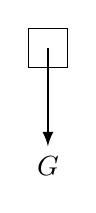
\begin{tikzpicture}[>=latex, scale=1]
       \draw(0,0) rectangle (.5,.5);
       \draw[->,thick](.25,.25)--(.25,-1)node[below]{$G$};
       \tkzDrawPoint(.25,.25)
    \end{tikzpicture}
    \caption{}
    \end{minipage}
    \begin{minipage}[t]{0.25\textwidth}
    \centering
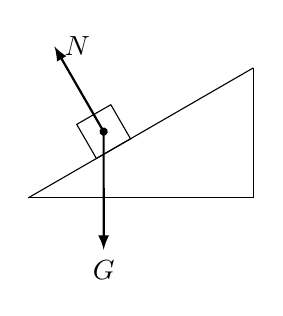
\begin{tikzpicture}[>=latex]
\draw [rotate=30] (0,0) rectangle (.5,.5);
\draw[rotate=30] (-1,0)--(2.3,0);
\fill[rotate=30] (.25,.25) circle[radius=1.5pt];
\draw[rotate=30, ->, thick](.25,.25)--(.25,1.5)node[right]{$N$};
\draw[rotate=30, ->, thick](.25,.25)--(-.5,.25-1.3)node[below]{$G$};
\draw(-.85,-.5)--(2,-.5)--(2,1.15);    
\end{tikzpicture}
    \caption{}
    \end{minipage}
    \begin{minipage}[t]{0.26\textwidth}
        \centering
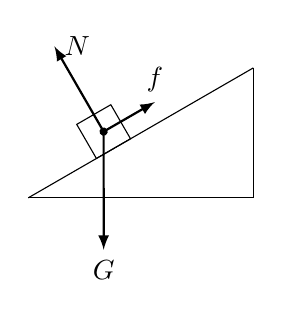
\begin{tikzpicture}[>=latex]
\draw [rotate=30] (0,0) rectangle (.5,.5);
\draw[rotate=30] (-1,0)--(2.3,0);
\fill[rotate=30] (.25,.25) circle[radius=1.5pt];
\draw[rotate=30, <->, thick](1,.25)node[above]{$f$}--(.25,.25)--(.25,1.5)node[right]{$N$};
\draw[rotate=30, ->, thick](.25,.25)--(-.5,.25-1.3)node[below]{$G$};
\draw(-.85,-.5)--(2,-.5)--(2,1.15);    
\end{tikzpicture}
        \caption{}
        \end{minipage}
            \begin{minipage}[t]{0.23\textwidth}
        \centering
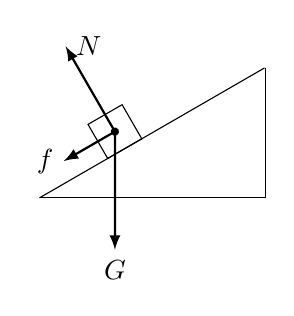
\begin{tikzpicture}[>=latex]
\draw [rotate=30] (0,0) rectangle (.5,.5);
\draw[rotate=30] (-1,0)--(2.3,0);
\fill[rotate=30] (.25,.25) circle[radius=1.5pt];
\draw[rotate=30, <->, thick](-.5,.25)node[left]{$f$}--(.25,.25)--(.25,1.5)node[right]{$N$};
\draw[rotate=30, ->, thick](.25,.25)--(-.5,.25-1.3)node[below]{$G$};
\draw(-.85,-.5)--(2,-.5)--(2,1.15);    
\end{tikzpicture}
        \caption{}
        \end{minipage}
    \end{figure}

\item 一个物体沿着光滑的斜面滑下来,物体受到几个力
的作用?物体原来具有某一速度,它沿着光滑的斜面滑上去的
时候受到几个力的作用?分别画出物体的受力图.

    如果物体和斜面之间有滑动摩擦,受力情况又怎样?再分
别画出物体的受力图.

\begin{solution}
    沿光滑斜面上滑或下滑都只受到重力和支持力这两
个力的作用(图1.19)。如果物体和斜面之间有滑动摩擦,物
体和斜面间就会有滑动摩擦力,斜面上的物体将受到重力、支
持力和滑动摩擦力这三个力的作用。下滑时,滑动摩擦力沿
斜面向上(图1.20),上滑时,滑
动摩擦力沿斜面向下(图1.21)。
\end{solution}
\item 雨滴下落的速度较大,空气阻力不能忽略不计.无
风的时候雨滴匀速竖直下落,雨滴受到几个力的作用?设雨滴
的重量是0.001牛,画出雨滴的受力图.

\begin{solution}
    雨滴受到重力和空气阻力的作用,由于雨滴匀速竖
    直下落,这两个力平衡,大小相等,方向相反。雨滴的受力图
    如图1.22所示.
\end{solution}
\item 用水平绳拉着木块在水平面上运动,木块的重量是
5牛,绳的拉力是10牛,滑动摩擦系数是0.3.画出木块的受力图.


\begin{solution}
    木块共受四个力:重力$G=5$牛,竖直向下;水平面
的支持力$N=5$牛,竖直向上;拉力$F=10$牛,方向水平;摩
擦力$f=0.3\x5=1.5$牛,方向与$F$相反,受力图如图1.23
所示。


\end{solution}

\begin{figure}[htp]\centering
    \begin{minipage}[t]{0.48\textwidth}
    \centering
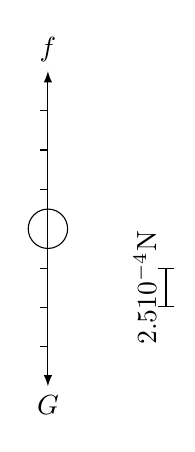
\begin{tikzpicture}[>=latex]
\draw(0,0) circle(0.25);
\draw[<->](0,2)node[above]{$f$}--(0,-2)node[below]{$G$};
\tkzDrawPoint(0,0)
\foreach \x in {-3,-2,-1,1,2,3}
{
    \draw(-.1,\x/2)--(0,\x/2);
}
\draw[|-|](1.5,-1)--node[rotate=90, above]{$2.5\x 10^{-4}$N}(1.5,-.5);
\end{tikzpicture}
    \caption{}
    \end{minipage}
    \begin{minipage}[t]{0.48\textwidth}
    \centering
\begin{tikzpicture}[>=latex]
    \draw[thick](-.2,-.2) rectangle (.2,.2);
    \draw[<->](-1,0)node[left]{$f$}--(5,0)node[right]{$F$};
\draw[<->](0,-2.5)node[right]{$G$}--(0,2.5)node[right]{$N$};
\foreach \x in {-1,1,2,...,9}
{
    \draw(\x/2,0)--(\x/2,-.1);
}
\foreach \x in {-4,-3,-2,-1,1,2,3,4}
{
    \draw(-.1,\x/2)--(0,\x/2);
}
\draw[|-|](2,2)--node[above]{1N}(2.5,2);
\end{tikzpicture}
    \caption{}
    \end{minipage}
    \end{figure}

\item 如课本图1.21那样用一根绳子$a$把物体挂起来,再用另一根
水平的绳子$b$把物体拉向一旁固定起来.这个物体受到几个力的
作用?画出物体的受力图.

\begin{solution}
    物体受到重力,绳子$a$和$b$对它的拉力三个力的
作用.受力图如图1.24所示.
\end{solution}

\item  在课本图1.16中没有画出书对桌面的压力$N'$,把这个力
画出来,并回答下面的问题:
\begin{enumerate}
\item 压力$N'$是什么性质的力?
\item 压力$N'$跟哪个力是一对作用力和反作用力?
\item 压力$N'$和重力$G$是不是作用在同一个物体上的力?
\item 在书静止地压在桌面上的情况下,压力$N'$和重力$G$的大小有什么关系?
\end{enumerate}

\begin{figure}[htp]\centering
    \begin{minipage}[t]{0.48\textwidth}
    \centering
\begin{tikzpicture}[>=latex]
\tkzDefPoints{0/0/O, -1.5/0/B, 0/-2/C, 1.5/2/A}
\draw(-.25,-.25) rectangle (.25,.25);
\draw[->, thick](O)--(A)node[above]{$F_a$};
\draw[->, thick](O)--(B)node[above]{$F_b$};
\draw[->, thick](O)--(C)node[right]{$F_c$};
\end{tikzpicture}
    \caption{}
    \end{minipage}
    \begin{minipage}[t]{0.48\textwidth}
    \centering
    \includegraphics[scale=.7]{fig/1-25.png}
    \caption{}
    \end{minipage}
    \end{figure}

\begin{solution}
    书对桌面的压力$N'$如图1.25所示.
\begin{enumerate}
\item 压力$N'$是弹力;    
\item 压力$N'$跟桌面对
书的支持力$N$是作用力和反作
用力;    
\item 压力$N'$和重力$G$不
是作用在同一物体上的力,$N'$作用在桌面上,$G$作用在书上;    
\item 书静止在桌面上时,压力
$N'$和重力$G$大小相等。
\end{enumerate}

\end{solution}
\end{enumerate}

\subsection{练习六}
\begin{enumerate}
\item 两个力的合力总大于原来的每一个力,这话对吗?为
什么?

\begin{solution}
    根据力的平行四边形法则,合力的大小由平行四边
形的对角线表示,原来两个力的大小由平行四边形的两个邻
边表示;而平行四边形的对角线并不总是大于其邻边的。所
以,“两个力的合力总大于原来的每一个力”的说法是不对的。
\end{solution}
\item 有两个力$F_1$和$F_2$,用作图法求出当它们之间的夹角
$\theta =0^\circ$, $30^\circ$, $60^\circ$, $90^\circ$, $120^\circ$, $150^\circ$, $180^\circ$时的合力.研究你所作
的图,能不能得到结论:夹角$\theta$在$0^\circ$到$180^\circ$之间时,$\theta $越大,合
力就越小.

\begin{solution}
    按照题中给出的各个夹角,用同一标度分别做出两
个力$F_1$和$F_2$的合力$R$, 如下列各图所示,测量$R$的大小,可
以得到结论:在$0^{\circ}$到$180^{\circ}$之间,夹角越大,合力就越小.

\begin{figure}[htp]\centering
    \begin{minipage}[t]{0.48\textwidth}
    \centering
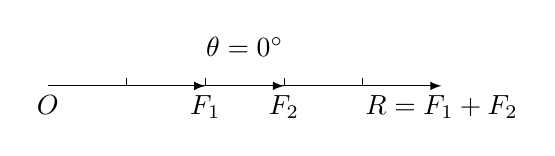
\begin{tikzpicture}[>=latex, scale=1]
\draw[->](0,0)node[below]{$O$}--(2,0)node[below]{$F_1$};
\draw[->](0,0)--(3,0)node[below]{$F_2$};
\draw[->](0,0)--(5,0)node[below]{$R=F_1+F_2$};
\node at (2.5,.5){$\theta=0^{\circ}$};
\foreach \x in {1,2,3,4}
{
    \draw(\x,0)--(\x,.1);
}
    \end{tikzpicture}
    \caption{}
    \end{minipage}
    \begin{minipage}[t]{0.48\textwidth}
    \centering
    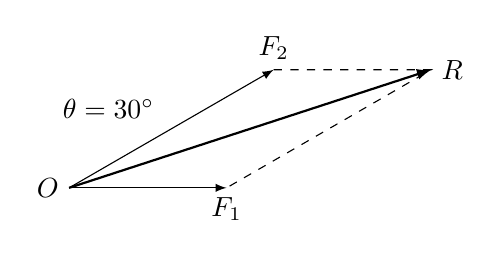
\begin{tikzpicture}[>=latex, scale=1]
\draw[->](0,0)--(2,0)node[below]{$F_1$};
\draw[->](0,0)--(30:3)node[above]{$F_2$};
\draw[dashed](30:3)--+(2,0)--(2,0);
\draw[thick,->](0,0)node[left]{$O$}--(4.6,1.5)node[right]{$R$};
\node at (0.5,1){$\theta=30^{\circ}$};

    \end{tikzpicture}
    \caption{}
    \end{minipage}
    \end{figure}

\begin{figure}[htp]\centering
    \begin{minipage}[t]{0.3\textwidth}
    \centering
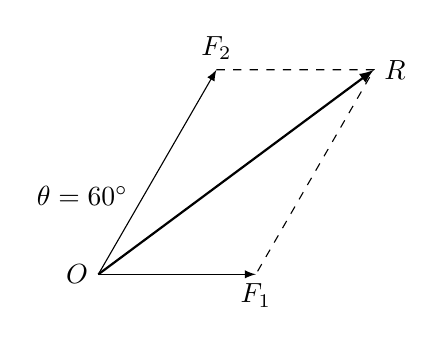
\begin{tikzpicture}[>=latex, scale=1]
    \draw[->](0,0)--(2,0)node[below]{$F_1$};
    \draw[->](0,0)--(60:3)node[above]{$F_2$};
    \draw[dashed](60:3)--+(2,0)--(2,0);
    \draw[thick,->](0,0)node[left]{$O$}--(1.5+2,1.5*1.732)node[right]{$R$};
    \node at (0.5,1)[left]{$\theta=60^{\circ}$}; 
    \end{tikzpicture}
    \caption{}
    \end{minipage}
    \begin{minipage}[t]{0.27\textwidth}
    \centering
    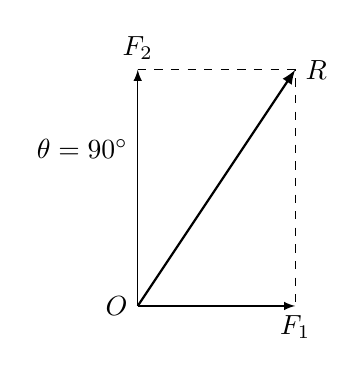
\begin{tikzpicture}[>=latex, scale=1]
    \draw[->](0,0)--(2,0)node[below]{$F_1$};
    \draw[->](0,0)--(90:3)node[above]{$F_2$};
    \draw[dashed](90:3)--+(2,0)--(2,0);
    \draw[thick,->](0,0)node[left]{$O$}--(2,3)node[right]{$R$};
    \node at (0,2)[left]{$\theta=90^{\circ}$};      
    \end{tikzpicture}
    \caption{}
    \end{minipage}
\begin{minipage}[t]{0.4\textwidth}
    \centering
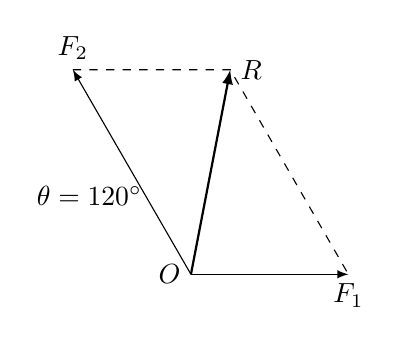
\begin{tikzpicture}[>=latex, scale=1]
    \draw[->](0,0)--(2,0)node[below]{$F_1$};
    \draw[->](0,0)--(120:3)node[above]{$F_2$};
    \draw[dashed](120:3)--+(2,0)--(2,0);
    \draw[thick,->](0,0)node[left]{$O$}--(-1.5+2,1.5*1.732)node[right]{$R$};
    \node at (-0.5,1)[left]{$\theta=120^{\circ}$};      
    \end{tikzpicture}
    \caption{}
    \end{minipage}
    \end{figure}

\begin{figure}[htp]\centering
    \begin{minipage}[t]{0.48\textwidth}
    \centering
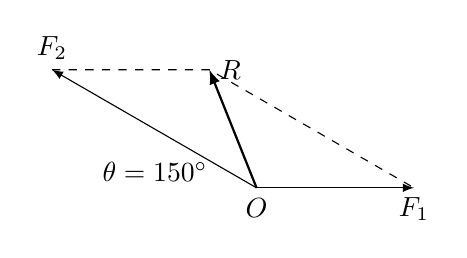
\begin{tikzpicture}[>=latex, scale=1]
    \draw[->](0,0)--(2,0)node[below]{$F_1$};
    \draw[->](0,0)--(150:3)node[above]{$F_2$};
    \draw[dashed](150:3)--+(2,0)--(2,0);
    \draw[thick,->](0,0)node[below]{$O$}--(-4.6+4,1.5)node[right]{$R$};
    \node at (-0.5,.2)[left]{$\theta=150^{\circ}$};      
    \end{tikzpicture}
    \caption{}
    \end{minipage}
    \begin{minipage}[t]{0.48\textwidth}
    \centering
    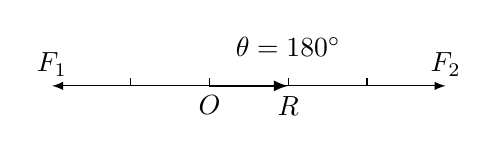
\begin{tikzpicture}[>=latex, scale=1]
      \draw[<->](-2,0)node[above]{$F_1$}--(0,0)node[below]{$O$}--(3,0)node[above]{$F_2$};
\draw[->, thick](0,0)--(1,0)node[below]{$R$};
\node at (1,.5){$\theta=180^{\circ}$};
\foreach \x in {-1,0,1,2}
{
    \draw(\x,0)--(\x,.1);
}
    \end{tikzpicture}
    \caption{}
    \end{minipage}
    \end{figure}

\end{solution}
\item 两个力的合力什么情况下最大,什么情况下最小?设
有两个力,一个是20牛,一个走5牛.合力的最大值是多大,最
小位是多大?

\begin{solution}
    当两个力间夹角$\theta=0^{\circ}$时合力最大,$\theta=180^{\circ}$时,合
力最小.合力的最大值$R_{\text{最大}}=20+5=25$牛;合力的最
小值$R_{\text{最小}}=20-5=15$牛.
\end{solution}
\item 2牛和10牛的两个力,它们的合力能够等于5牛、10牛、
15牛吗?

\begin{solution}
    2牛和10牛的两力,合力的最小值为$10-2=8$牛,合力的最大值为$10+2=12$牛.所以这两个力
的合力不能等于5牛和15牛,可以等于10牛.
\end{solution}
\item   两个力互成$30^\circ$角, 大小分别是90牛和120牛.用作图法求出合力的
大小和方向,然后再用公式来求.

\begin{figure}[htp]
    \centering
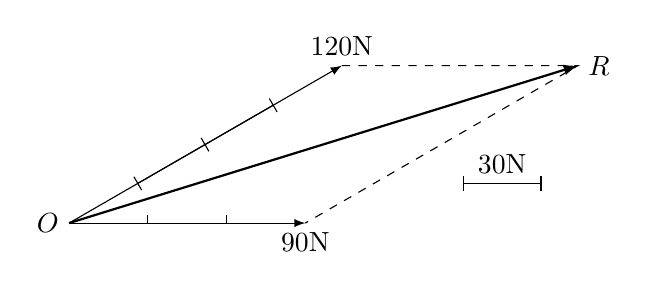
\begin{tikzpicture}[>=latex, scale=1]
    \draw[->](0,0)--(3,0)node[below]{90N};
    \draw[->](0,0)--(30:4)node[above]{120N};
    \draw[dashed](30:4)--+(3,0)--(3,0);
    \draw[thick,->](0,0)node[left]{$O$}--(2*1.732+3, 2)node[right]{$R$};
\draw[|-|](5,.5)--node[above]{30N}(6,.5);
\foreach \x in {1,2}
{
    \draw(\x,0)--(\x,.1);
}
\draw[|-|](30:2)--(30:1);
\draw[-|](30:2)--(30:3);
\end{tikzpicture}
    \caption{}
\end{figure}


\begin{solution}
    利用平行四边形法则作图得合力$R$如图1.33所示。
按照标度测量$R$的长度,得合力的大小为204牛.用量角器
测得合力与90牛的力的夹角为$17^{\circ}$.

利用公式,合力的大小
\[R=\sqrt{90^2+120^2+2\x90\x120\cos30^{\circ}}=203{\rm N}\]
合力与90牛的力的夹角的正切
\[\tan\phi = \frac{120\sin 30^{\circ}}{90+120\cos30^{\circ}}=
0.31\]
查表得$\phi=17^{\circ}$.
\end{solution}
\end{enumerate}


\subsection{练习七}
\begin{enumerate}

\item 一个物体的重量是20牛,把它放在一个斜面上,斜面
长$AB$与斜面高$BC$之比是$5:3$.把重力分解,求出平行于斜面
使物体下滑的力和垂直于斜面使物体压紧斜面的力.
 \begin{figure}[htp]\centering
    \begin{minipage}[t]{0.48\textwidth}
    \centering
\includegraphics[scale=.6]{fig/1-34.png}
    \caption{}
    \end{minipage}
    \begin{minipage}[t]{0.48\textwidth}
    \centering
    \includegraphics[scale=.6]{fig/1-35.png}
    \caption{}
    \end{minipage}
    \end{figure}

\begin{solution}
根据题意作图1.34. 平行于斜面使物体下滑的力
\[F_1=\frac{BC}{AB}G=\frac{3}{5}\x 20{\rm N}=12{\rm N}\]
垂直于斜面使物体压紧斜面的力
\[F_2=\frac{AC}{AB}G=\frac{4}{5}\x20{\rm N}=16{\rm N}\]    
\end{solution}


\item 图1.35是塔式起重机,钢索$NO$与水平悬臂$MO$成
$30^\circ$角,当起重机吊着$4.0\times 10^4$牛的货物时,钢索和悬臂分别受
多大的力?
 
\begin{solution}
    根据题意得知$F=4.0\x10^4$牛.从图得钢索受的力
\[F_1=\frac{F}{\sin 30^{\circ}}=\frac{4.0\x10^4}{0.50}=8.0\x10^4{\rm N}\]
悬臂受的力
\[F_2=\frac{F}{\tan 30^{\circ}}=\frac{4.0\x10^4}{0.577}=6.9\x10^4{\rm N}\]
\end{solution}
\item 如图1.36所示,垂直作用在帆上的风力$F=1.0\times 10^4$
牛.沿着船身方向的分力$F_1$使帆船前进,垂直于船身方向的
分力$F_2$使船身侧倾.设$F$与船身方向成$45^\circ$角,求力$F_1$是多大.
\begin{figure}[htp]\centering
    \begin{minipage}[t]{0.48\textwidth}
    \centering
       \includegraphics[scale=.7]{fig/1-36.png}
    \caption{}
    \end{minipage}
    \begin{minipage}[t]{0.48\textwidth}
    \centering
    \begin{tikzpicture}[>=latex, scale=.8]
\tkzDefPoints{0/0/F2, 4/0/G, 4/3/O, 8/3/F1}
\draw[->, thick](O)node[above]{$O$}--(F2)node[below]{$F_2$};
\draw[->, thick](O)--(G)node[right]{$G=180$N};
\draw[->, thick](O)--(F1)node[right]{$F_1$};
\draw[dashed](F1)--(G)--(F2);
\draw[|-|](0,2)--node[above]{60N}(1,2);
\foreach \x in {1,2}
{
    \draw(4+\x,3+0)--(4+\x,3+.1);
    \draw(4+0,\x)--(4+.1,\x);
}
\draw(7,3)--(7,3.1);

\foreach \x in {1,3}
{
    \draw[|-|](36.87:\x)--(36.87:\x+1);
}
\tkzMarkAngle[mark=none, size=.6](F2,O,G)
\tkzMarkRightAngle[mark=none, size=.3](G,O,F1)
\tkzLabelAngle(F2,O,G){$\theta$}
    \end{tikzpicture}
    \caption{}
    \end{minipage}
    \end{figure}

\begin{solution}
    由图可以看出沿着船身方
向的分力
\[F_1=F\cos45^{\circ}=1.0\times 10^4\x \frac{\sqrt{2}}{2}=7.1\times 10^3{\rm N}\]
\end{solution}

\item 把竖直向下的180牛的力分解为两个分力,一个分力
在水平方向上并等于240牛,求另一个分力的大小和方向.

 
\begin{solution}
    根据题意作图,如图1.37所示,$G=180$牛,$F_1=240$牛,则另一个分力的大小
 \[   F_2=\sqrt{G^2+F_1^2}=\sqrt{180^2+240^2}=300{\rm N}\]

 $F_2$和$G$夹角的余弦
 \[\cos\theta=\frac{G}{F_2}=\frac{180{\rm N}}{300{\rm N}}=0.6\]

 所以夹角$\theta=53^{\circ}8'$, 即$F_2$的方向和竖直向下的方向成
$53^{\circ}8'$的角.
\end{solution}
\item 一个小同学跟一个大同学拔河,小同学拉不动大同
学,可是用下述办法,小同学就可以拉动大同学.在树干上
拴一条绳子,大同学拿着绳子的另一端,沿水平方向把绳子拉
紧.小同学用力推绳子的中点,就可以拉动大同学了.实际
做一做,并解释所发生的现象.

\begin{figure}[htp]
    \centering
\includegraphics[scale=.8]{fig/1-38.png}
    \caption{}
\end{figure}

 \begin{solution}
    图1.38是根据题意画的示意图。小同学推绳子
    的力为$F$,大同学受到的拉力是$F$的一个分力$F_1$
\[F_1=\frac{F}{2\cos\frac{\theta}{2}}\]
 $\theta$   是两段绳子间的夹角。当角$\theta$接近$180^{\circ}$时,$\cos\frac{\theta}{2}$
    接近于零,分力$F_1$比小同学用力$F$大得多,所以能拉动大同学。
\end{solution}
\end{enumerate}

\subsection{习题}

\begin{enumerate}
\item   如图1.39所示,为了防止电线杆倾倒,常在两侧对称
地拉上钢绳.如果两条钢绳间的夹角是$60^\circ$,每条钢绳的拉力
都是300牛,求两条钢绳作用在电线杆上的合力.

\begin{figure}[htp]
\centering
\begin{minipage}[t]{0.48\textwidth}
\centering
\begin{tikzpicture}[>=stealth,  thick, scale=.7]

\fill [pattern = north east lines] (-3,-.25) rectangle (3,0);
\draw(-3,0)--(3,0);


\draw (0,4.5)--(-2.5,0);
\draw (0,4.5)--(2.5,0);
\foreach \x in{1,2,3}
{
    \draw [fill=white] (-.5,4.8+\x*0.2) rectangle (.5,4.8+\x*0.2+.1);
}
\draw [fill=white] (-.1,0) rectangle (.1,6);


\draw [->](-1.4,3)--(-2,2);
\draw [->](1.4,3)--(2,2);
\end{tikzpicture}
\caption{}
\end{minipage}
\begin{minipage}[t]{0.48\textwidth}
\centering
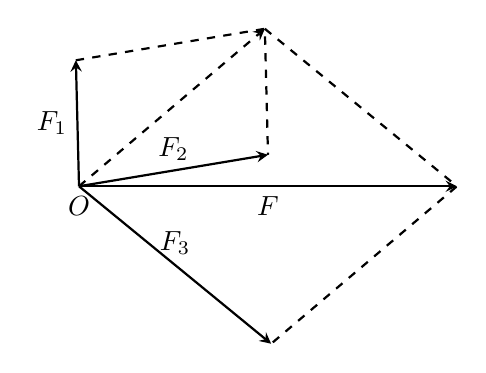
\begin{tikzpicture}[>=stealth,  thick, scale=.8]

\draw [->] (0,0)node [below]{$O$}--node [below]{$F$}(6,0);
\draw [->] (0,0)--node [left]{$F_1$}(-.05, 2);
\draw [->] (0,0)--node [above]{$F_2$}(3, .5);
\draw [dashed] (-.05, 2)--(-.05+3, 2.5)--(3, .5);
\draw [dashed] (-.05+3, 2.5)--(6,0)--(6-3+.05, -2.5);
\draw [->,dashed] (0,0)--(-.05+3, 2.5);
\draw [->] (0,0)--node [above]{$F_3$} (6-3+.05, -2.5);
\end{tikzpicture}
\caption{}
\end{minipage}
\end{figure}

\begin{solution}
    解法一:根据力的平行四边形法则
\[\begin{split}
    F&=\sqrt{F^2_1+F^2_2+2F_1F_2\cos\theta}\\
    &=\sqrt{300^2+300^2+2\x300\x300\cos60^{\circ}}\\
    &=300\sqrt{3}=519{\rm N}
\end{split}\]
方向竖直向下.

    解法二:由于$F_1=F_2$, 这一平行四边形是一个菱形
    \[F=2F_1\cos\frac{\theta}{2}=2\x300\x\cos\frac{60^{\circ}}{2}=300\sqrt{3}=519{\rm N}\]
    方
    向竖直向下。
\end{solution}
\item  图1.40表示用平行四边形法则求三个共点力$F_1$、$F_2$、$F_3$
的合力$F$.先求出$F_1$和$F_2$的合力,再求出这个合力与$F_3$的
合力$F$.改用三角形法求出这三个力的合力.改变求和的顺
序,再分别用平行四边形法则和三角形法求出这三个力的合
力.

\begin{solution}
用三角形法求$F_1$、$F_2$、$F_3$的合力$F$如图1.41所示。
图中$F'$是$F_1$、$F_2$的合力.
\begin{figure}[htp]\centering
    \begin{minipage}[t]{0.48\textwidth}
    \centering
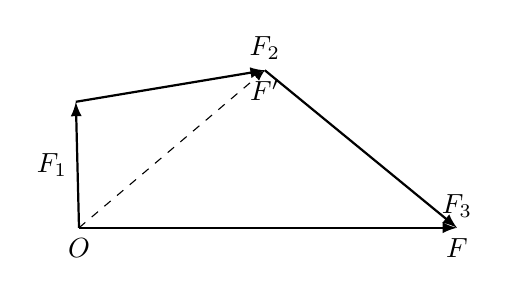
\begin{tikzpicture}[>=latex, scale=.8]
\draw [->, thick] (0,0)node [below]{$O$}--(6,0)node [below]{$F$};
\draw [->, thick] (0,0)--node [left]{$F_1$}(-.05, 2);
\draw [->, thick] (-.05, 2)--+(3, .5)node [above]{$F_2$};
\draw [->, thick] (-.05+3, 2.5)--+(6-3+.05, -2.5)node [above]{$F_3$} ; 
\draw [->,dashed] (0,0)--(-.05+3, 2.5)node [below]{$F'$};
    \end{tikzpicture}
    \caption{}
    \end{minipage}
    \begin{minipage}[t]{0.48\textwidth}
    \centering
    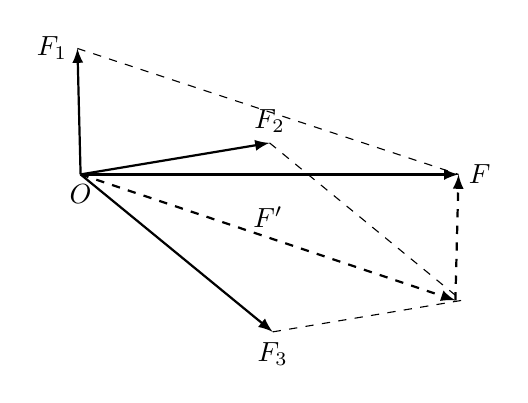
\begin{tikzpicture}[>=latex, scale=.8]
\draw [->, thick] (0,0)node [below]{$O$}--(6,0)node [right]{$F$};
\draw [->, thick] (0,0)--(-.05, 2)node [left]{$F_1$};
\draw [->, thick] (0,0)--(3, .5)node [above]{$F_2$};
\draw [->, thick] (0,0)-- (6-3+.05, -2.5)node [below]{$F_3$};
\draw [dashed] (-.05, 2)--(6,0);
\draw [dashed] (3, .5)--+(6-3+.05, -2.5)--(6-3+.05, -2.5);
\draw [->,dashed, thick] (0,0)--node[above]{$F'$}(5.95,-2);
\draw [->,dashed, thick] (5.95,-2)--(6,0);
    \end{tikzpicture}
    \caption{}
    \end{minipage}
    \end{figure}

改变求和的顺序,用平行四边形法则求这三个力的合力,
如图1.42所示,即先求$F_2$、$F_3$的合力$F'$, 再求$F'$、$F_1$的合
力,即三个力的合力$F$.

改变求和的顺序,用三角形法求这三个力的合力,如图1.
43所示,即先求$F_2$、$F_3$的合力$F'$, 再求$F'$, $F_1$的合力,即三个力的合力$F$.
\end{solution}

\begin{figure}[htp]\centering
    \begin{minipage}[t]{0.48\textwidth}
    \centering
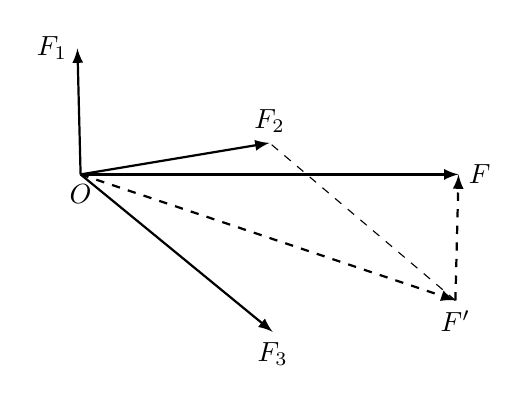
\begin{tikzpicture}[>=latex, scale=.8]
\draw [->, thick] (0,0)node [below]{$O$}--(6,0)node [right]{$F$};
\draw [->, thick] (0,0)--(-.05, 2)node [left]{$F_1$};
\draw [->, thick] (0,0)--(3, .5)node [above]{$F_2$};
\draw [->, thick] (0,0)-- (6-3+.05, -2.5)node [below]{$F_3$};

\draw [->,dashed, thick] (0,0)--(5.95,-2)node[below]{$F'$};
\draw [dashed] (5.95,-2)--(3, .5);
\draw [->,dashed, thick] (5.95,-2)--(6,0);
    \end{tikzpicture}
    \caption{}
    \end{minipage}
    \begin{minipage}[t]{0.48\textwidth}
    \centering
    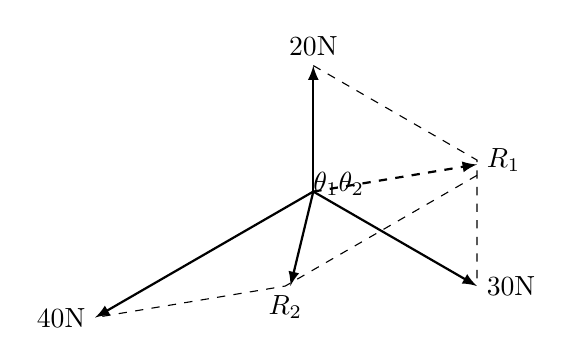
\begin{tikzpicture}[>=latex, scale=.8]
\foreach \x/\y in {90/2, -30/3, -150/4}
{
    \draw[->,thick] (0,0)--(\x:\y);
}   
\draw[dashed](0,2)--+(-30:3)node(R1)[right]{$R_1$}--(-30:3);
\draw[->,thick, dashed](0,0)--(R1);
\draw[dashed](R1)--+(-150:4)node(R2)[below]{$R_2$}--(-150:4);
\draw[->,thick](0,0)--(R2);

\node at (90:2)[above]{20N};
\node(A) at (-30:3)[right]{30N};
\node(B) at (-150:4)[left]{40N};
\tkzDefPoints{0/0/O}
\tkzMarkAngles[mark=none, size=.6](A,O,R1 B,O,R2)
\tkzLabelAngle(A,O,R1){$\theta_1$}
\tkzLabelAngle(B,O,R2){$\theta_2$}
    \end{tikzpicture}
    \caption{}
    \end{minipage}
    \end{figure}



\item   20牛、30牛和40牛的三个力作用于物体的一点,它们
之间的夹角都是$120^\circ$.求合力的大小和方向.

\begin{solution}
根据题意画出受力图,如图1.44所示.先合成20
牛和30牛二力得$R_1$, 再将$R_1$和40牛合成得$R_2$
\[R_1=\sqrt{20^2+30^2+2\x20\x30\cos120^{\circ}}=10\sqrt{7}=26.5{\rm N}\]
\[\tan\theta_1=\frac{20\sin 120^{\circ}}{30+20\cos 120^{\circ}
}=0.866,\qquad \theta_1=41^{\circ}\]
\[R_2=\sqrt{40^2+(10\sqrt{7})^2+2\x40\x10\sqrt{7}\cos(120^{\circ}+\theta_1)}=17.3{\rm N}\]
\[\tan\theta_2=\frac{26.5\sin 161^{\circ}}{40+26.5\cos161^{\circ}}=0.577,\qquad \theta_2=30^{\circ}\]


\end{solution}
\item 如图1.45所示,把一个重量为10牛的物体挂在绳子
上,已知$AC=BC=3$米,$CD=1$米.求绳$AC$和$BC$所受的拉
力.
\begin{figure}[htp]
\centering
\begin{tikzpicture}[>=stealth,  thick, scale=.8]

\fill [pattern = north east lines] (-4.1,-.5) rectangle (-3.8,.5);
\draw(-3.8,.5)--(-3.8,-.5);
\fill [pattern = north east lines] (4.1,-.5) rectangle (3.8,.5);
\draw(3.8,.5)--(3.8,-.5);

\draw [dashed] (-3.8,0)  --node[above]{$D$} (3.8,0);
\node at (-3.5,0) [below]{$A$};
\node at (3.5,0) [below]{$B$};
\draw [dashed] (0,0)  -- (0,-1.5)node[above]{$C$};
\draw  (0,-1.5)  -- (0,-2.5);
\draw (-3.8,0)--(0,-1.5)--(3.8,0);
\draw [fill=black!30] (-.5,-2.5) rectangle (.5,-2.75-.6);


\end{tikzpicture}
\caption{}
\end{figure}


\begin{solution}
    根据题意画受力图,如图1.46所示,由图得
\[\frac{AC}{DC}=\frac{F_{AC}}{\frac{1}{2}G}\]
所以绳$AC$所受的拉力
\[F_{AC}=\frac{G}{2}\cdot \frac{AC}{DC}=\frac{10}{2}\x 3=15{\rm N}\]
绳$BC$所受的拉力
\[F_{BC}=F_{AC}=15{\rm N}\]
\end{solution}

\begin{figure}[htp]\centering
    \begin{minipage}[t]{0.48\textwidth}
    \centering
\begin{tikzpicture}[>=latex, scale=1.4]
    \fill [pattern = north east lines] (-2,-.5) rectangle (-1.8,.5);
    \draw(-1.8,.5)--(-1.8,-.5);
    \fill [pattern = north east lines] (2,-.5) rectangle (1.8,.5);
    \draw(1.8,.5)--(1.8,-.5);
\draw[dashed](-1.8,0)--(1.8,0);
\draw[dashed](1.5,-1.5)--(-1.5,-1.5);
\draw[dashed](0,0)--(0,-1);
\draw[->, thick](0,-.8)--(0,-2.2)node[below]{$G$};
\draw[dashed](-1.5,-1.5)--(0,-2.2)--(1.5,-1.5);
\draw[->, thick](-1.8,0)--(1.5,-1.5)node[right]{$F_{AC}$};
\draw[->, thick](1.8,0)--(-1.5,-1.5)node[left]{$F_{BC}$};
\node at (.2,-1.5)[above]{$E$};
\node at (.2,-.7)[above]{$C$};\node at (0,0)[above]{$D$};
\node at (1.6,0)[below]{$B$};\node at (-1.6,0)[below]{$A$};
\end{tikzpicture}
    \caption{}
    \end{minipage}
    \begin{minipage}[t]{0.48\textwidth}
    \centering
    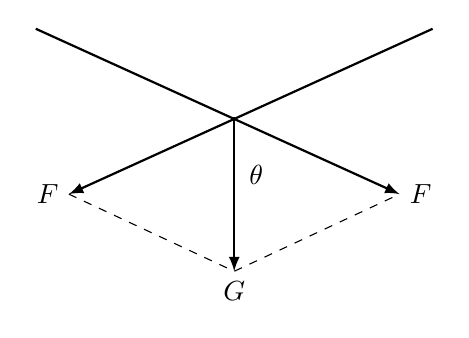
\begin{tikzpicture}[>=latex, scale=1.4]
\draw[->, thick](-1.8,0)--(1.5,-1.5)node(B)[right]{$F$};
\draw[->, thick](1.8,0)--(-1.5,-1.5)node(C)[left]{$F$};
\draw[->, thick](0,-.8)node(A){}--(0,-2.2)node[below]{$G$};
\draw[dashed](-1.5,-1.5)--(0,-2.2)--(1.5,-1.5);
\tkzMarkAngle[mark=none, size=.3](C,A,B)
\node at (.2,-1.5)[above]{$\theta$};
    \end{tikzpicture}
    \caption{}
    \end{minipage}
    \end{figure}

\item   用手握着橡皮绳的两端,在橡皮绳的中间挂一个重
物,当两手之间的距离增大或减小的时候,物体对橡皮绳的
拉力是否改变?怎样改变?实际做一下,并说明道理.


\begin{solution}
    要改变,道理如下:如图1.47所示,重物$G$挂在绳中
    间,可看成在绳中间加一拉力,拉力的大小等于重物所受的重
    力,这个拉力可按平行四边形法则分解成两个分力$F$, 当两
    手拉开时,两个分力的夹角$\theta$增大,两个分力也随之增大.

    说明:这个问题还可以做一些定量分析。由于
    \[G^2=F^2+F^2+2F\cdot F\cos\theta\]
    因此:
    \[F=\sqrt{\frac{1}{2(1+\cos\theta)}}\cdot G\]
    当$90^{\circ}<\theta<180^{\circ}$时,$\cos\theta$为负值,$\theta$越大,$|\cos\theta|$越大,$F$也
    随之增大。
\end{solution}
\item  刀、斧、凿、刨等切削工具的刃部叫做劈,劈的纵截面
是一个三角形,如图1.48所示.使用劈的时候,在劈背上加力
$F$,这个力产生两个效果,这就是使劈的两个侧面推压物体,
把物体劈开.设劈的纵截面是一个等腰三角形,劈背的宽度
是$d$,劈的侧面的长度是$\ell$,可以证明:
\[f_1=f_2=\frac{\ell}{d}F \]

从上式可知,当$F$一定的时侯,劈的两个侧面之间的夹角
越小,$\ell/d$就越大,$f_1$和$f_2$就越大.这说明了为什么越锋利的
切削工具越容易劈开物体.试证明上式.
\begin{figure}[htp]\centering
    \begin{minipage}[t]{0.48\textwidth}
    \centering
\includegraphics[scale=.6]{fig/1-48.png}
    \caption{}
    \end{minipage}
    \begin{minipage}[t]{0.48\textwidth}
    \centering
    \includegraphics[scale=.6]{fig/1-49.png}
    \caption{}
    \end{minipage}
    \end{figure}


\begin{solution}
    如图1.48所示,$f_1$、$f_2$是$F$的两个分力,由于三角
    形$ABC$与三角形$OPQ$相似,则有
\[\frac{f_1}{F}=\frac{\ell}{d}\]
因此:\[f_1=f_2=\frac{\ell}{d}F\]
\end{solution}


\item 一个物体放在倾角为$\theta$的光滑斜面上,求物体受到
的合力.

\begin{solution}
    略(课本已作解答)。
\end{solution}
   

\item 一个滑雪人沿着山坡滑下.滑雪人的重量是700牛,
山坡的倾角是$30^\circ$,滑雪板和雪地的滑动摩擦系数是0.04.求
滑雪人所受的合力.

\begin{solution}
如图1.49所示,滑雪人所受的重力$G$分解为平行于
山坡的分力$F_1$和垂直于山坡的分力$F_2$。

在垂直于山坡方向上,滑
雪人受到的重力的分力$F_2$和
山坡的支持力,两者大小相等,
方向相反,合力为零。

在平行于山坡方向上,滑
雪人受到重力的分力$F_1$和相
反方向的摩擦力$f$。
\[\begin{split}
   F_1&=G \sin 30^{\circ} =700\x\frac{1}{2}=350{\rm N}\\
   f&=\mu N=\mu F_2=\mu G\cos 30^{\circ}=0.04\x700\x\frac{\sqrt{3}}{2}=24{\rm N}
\end{split}\]
所以滑雪人受到的
合力$F=F_1-f=350-24=326$牛.方向平行于山坡、
向下。
\end{solution}
\end{enumerate}






















































































\section{参考资料}
\subsection{四种基本的力}
按照现代物理学的观点,自然界存在
四种基本的相互作用:万有引力(简称引力)、电磁力、强相互
作用力和弱相互作用力,在宏观世界里能显示其作用
的只有两种,即引力和电磁力。这两种力是长程力,它们的
作用范围从理论上说是无限的。强相互作用和弱相互作用则
是短程力,强作用力只在$10^{-15}$米范围内才有显著作用;弱
作用的力程更短,不超过$10^{-16}$米,这两种力只有在原子核内
部和基本粒子的相互作用中才显示出来,在宏观世界里不能
察觉它们的存在。

四种相互作用,按其作用的强弱次序排列,依次为:强相
互作用、电磁相互作用、弱相互作用、引力相互作用。一对质
子在相距$10^{-15}$米时,各种相互作用的相对强度为
\begin{center}
    \begin{tabular}{p{.25\textwidth}l}
  强相互作用&1\\
电磁相互作用&$10^{-2}$\\
弱相互作用&$10^{-14}$\\
引力相互作用&$10^{-40}$ 
    \end{tabular}
\end{center}

尽管四种相互作用的差别如此巨大,仍然有一些物理学
家致力于寻求各种相互作用的统一理论,近年来,在弱作用和
电磁作用的统一方面,已取得成功,实验已经证明,正如电和
磁是电磁作用的两种不同表现一样,弱作用和电磁作用也只
不过是统一的弱电相互作用的两种不同表现而已。

值得注意的是自然界中是否还有新的未被发现的基本作
用力呢?这个问题也有人在研究。最近发表的研究报告表明,
可能有第五种力存在。这种力在影响落体的加速度方面起着
跟引力相反的作用。它的相对强度可能只有引力作用的百分
之一,作用范围只有几百米,是一种中程力。

\subsection{力的等效移动}

作用在物体上的力,可以用有向线段
来表示,有向线段应当从力的作用点画起。但实际上,在对物
体进行受力分析时,常常把力的作用点沿着力的作用线移动
或者把力在物体上平移,而不改变力的作用效果。

\begin{figure}[htp]
    \centering
\includegraphics[scale=.45]{fig/1-50.png}
    \caption{}
\end{figure}

在外力作用下,形状和体积都不起变化的物体叫刚体。
作用在刚体上的可以沿着力的作用线的方向移到任意一点
而不改变力的效果。力的这种性质,叫做刚体内的力的可传
性.这一性质可以用图1.50来说明,甲图表示刚体的$A$点
受一外力$F_A$. 乙图表示再在$F$的作用线上任意一点$B$附加
一对平衡力$F_B$和$F_{B'}$, 这样并不会改变刚体的运动状态。如:
果使附加的平衡力$F_B$、$F_{B'}$的大小和$F_A$的大小相等,这时
$F_{B'}$和$F_{A}$也是一对平衡力;于是,去掉这对平衡力对刚体的
运动状态也没有影响,如图丙所示。可见,作用在刚体$A$点的
力$F_A$被作用在$B$点的力$F_B$等效代替,这样的效果就相当于
$F_A$沿其作用线从$A$点移到了$B$点。

一切实际物体都不是刚体,但是一般固体在外力作用下
发生的形变并不显著,可以近似看成刚体。中学研究物体
受力时,实际上是把物体看成是质点或近似看成刚体来做受
力图的。

这里再说明一下力的平移。研究平面上的物体在重力
$G$、支持力$N$、拉力$F$和摩擦力$f$作用下保持平衡时,受力图
常使$G$、$N$、$F$、$f$交于一点,如图1.51所示.
\begin{figure}[htp]\centering
    \begin{minipage}[t]{0.48\textwidth}
    \centering
\begin{tikzpicture}[>=latex, scale=1]
\fill[pattern=north east lines](-1.5,-.2) rectangle (1.5,0);
\draw(-1.5,0)--(1.5,0);
\draw (-.7,0) rectangle(.7,1);
\draw[<->, thick](-1.2,.5)node[left]{$f$}--(1.2,.5)node[right]{$F$};
\draw[<->, thick](0,-1)node[below]{$G$}--(0,2)node[above]{$N$};
\tkzDrawPoint(0,.5)
    \end{tikzpicture}
    \caption{}
    \end{minipage}
    \begin{minipage}[t]{0.48\textwidth}
    \centering
    \begin{tikzpicture}[>=latex, scale=1]
\fill[pattern=north east lines](-2.5,-.2) rectangle (2.5,0);
\draw(-2.5,0)--(2.5,0);
\draw (-.7,0) rectangle(.7,1);
\draw[->, thick](-.7,0)node[below]{$A$}--(-1.5,0)node[above]{$f$};
\draw[->, thick](0,.5) --(1.2,.5)node[right]{$F$};
\draw[->, thick](0,.5) -- (0,-1)node[below]{$G$};
\node at (.7,0) [below]{$B$};
\draw[dashed](-2,.5)--(0,.5)--(0,2.3);
\draw[<->](-1.8,0)--node[left]{$d_1$}(-1.8,.5);
\draw[->, thick](.4,0)--(.4,1.5)node[right]{$N$};
\draw[dashed](.4,1.5)--(.4,2.3);
\draw[<->](0,1.8)--node[above]{$d_2$}(.4,1.8);
\tkzDrawPoint(0,.5)      
    \end{tikzpicture}
    \caption{}
    \end{minipage}
    \end{figure}

这样做在许多情况下是把物体看成质点来研究的。而实
际的物体受力图应如图1.52所示.这时,拉力$F$和摩擦力$f$
是一对力偶,力偶矩$M_1=fd_1$, 这个力偶矩使物体沿顺时针
方向转动;重力$G$和支持力$N$是另一对力偶,其力偶矩$M_2
=Nd_2$, 这个力偶矩使物体沿逆时针方向转动.物体之所以
没有转动,是因为这两对力偶矩相互平衡,即$fd_1=Nd_2$. 这
是物体在$G$、$N$、$F$、$f$四个力作用下保持平衡的一个条件。
另一个条件是:$F=f$, $G=N$. 从$fd_1=Nd_2$这一平衡条件可以
看出,当静摩擦力$f$随外力增大时,$d_2$也相应地增大才能保
持平衡.若$d_2$已增大到无法再增大时,如图中$d_2=AB/2$
时,就能
使$fd_1>Nd_2$, 这时物体将以$B$为轴沿顺时针方向转动。当然
静摩擦力$f$的增大也有个最大限度$f_m=\mu_0 N$. 当$f$增大到
$f_m$ 仍然不能使$f_md_1>Nd_2$时,物体就不会转动.

在图1.52的分析中考虑到物体受力时可能产生的转动。
如果实际问题表明,物体受力后不会有转动,则把图1.52简
化为图1.51并不影响力的作用效果。这就是我们在研究物体
受力平衡时,可以用图1.51来代替图1.52的原因.

上面是就物体受到几个力保持平衡状态的情况而说的。
事实上,只要物体受力后会有转动,都可以将受力图简化,
把几个力绘成交于一点,而不改变原来力的作用效果。

更一般的情况而言,力也可以平移,但要满足力的平移原
理,即把作用在物体上的力平行于它的作用线移到物体上任
意一点而不改变原来力对物体的作用效果,则必须附加一个
力偶,这个力偶产生的力偶矩等于原来的力对这一点的力矩。

\subsection{关于塔式起重机的简单说明}

课本图1.31是塔式起重机。图中钢索$NO$是用来改变
起重臂(悬臂)仰角的,它属于起重机的变辐机构,由装在平衡
臂上的电动卷扬机牵引,图中悬挂重物的钢索是用来起重的,
它属于起重机的起升机构,由装在塔身中部的电动卷扬机牵
引。钢索$NO$的拉力和起重钢索的拉力大小是不同的。起重
机悬臂(起重臂)$MO$与塔身是铰链连接,悬臂仰角可以改变。
而不是固接在塔身上不能动的。


